\documentclass[notes=show]{beamer}
\usepackage{mathpazo}
\usepackage{hyperref}
\usepackage{multimedia}
\usepackage{tcolorbox}
\usepackage{tikz}
\usetikzlibrary{shadows}
\usetheme{metropolis}
\usecolortheme{default}
\setbeamertemplate{itemize item}{%
    
\begin{tikzpicture}
        \shade[ball color=black!100!yellow, preaction={fill=black,
opacity=.00,transform canvas={xshift=1mm,yshift=-1mm, yscale=0.5}}] (0,0) circle (0.6ex);
    \end{tikzpicture}
}
\setbeamertemplate{itemize subitem}{%
    
\begin{tikzpicture}
        \shade[ball color=black!100!white, preaction={fill=black,
        opacity=.00,transform canvas={xshift=1mm,yshift=-1mm, yscale=0.5}}] (0,0) circle (0.6ex);
    \end{tikzpicture}
}
\setbeamercolor{frametitle}{bg=white}
\setbeamercolor{frametitle}{fg=black}
\setbeamercolor{background canvas}{bg=white}
\setbeamercolor{block body}{bg=mDarkTeal!30}
\setbeamercolor{block title}{bg=mDarkTeal,fg=black!2}
\setbeamertemplate{navigation symbols}{}
\setbeamertemplate{footline}[page number]
\newenvironment{stepenumerate}{\begin{enumerate}[<+->]}{\end{enumerate}}
\newenvironment{stepitemize}{\begin{itemize}[<+->]}{\end{itemize} }
\newenvironment{stepenumeratewithalert}{\begin{enumerate}[<+-| alert@+>]}{\end{enumerate}}
\newenvironment{stepitemizewithalert}{\begin{itemize}[<+-| alert@+>]}{\end{itemize} }

\begin{document}

\title{Automation and New Tasks: How Technology Displaces and Reinstates Labor}
\subtitle{}
\date{Daron Acemoglu \& Pascual Restrepo \bigskip \\
\textit{Journal of Economic Perspectives}, Spring 2019}
\author{}
\maketitle

\newpage
\begin{center}
\begin{figure}
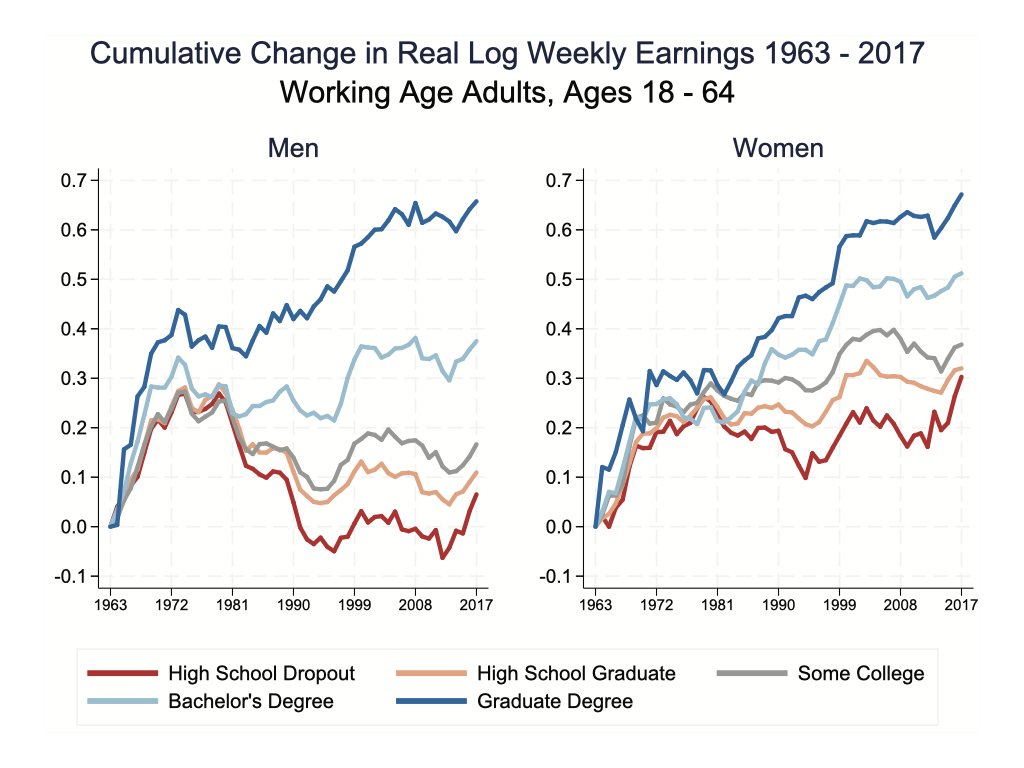
\includegraphics[height=8.5cm,width=\textwidth]{figureM1.png} 
\end{figure}
\end{center}
\newpage

\newpage
\begin{center}
\begin{figure}
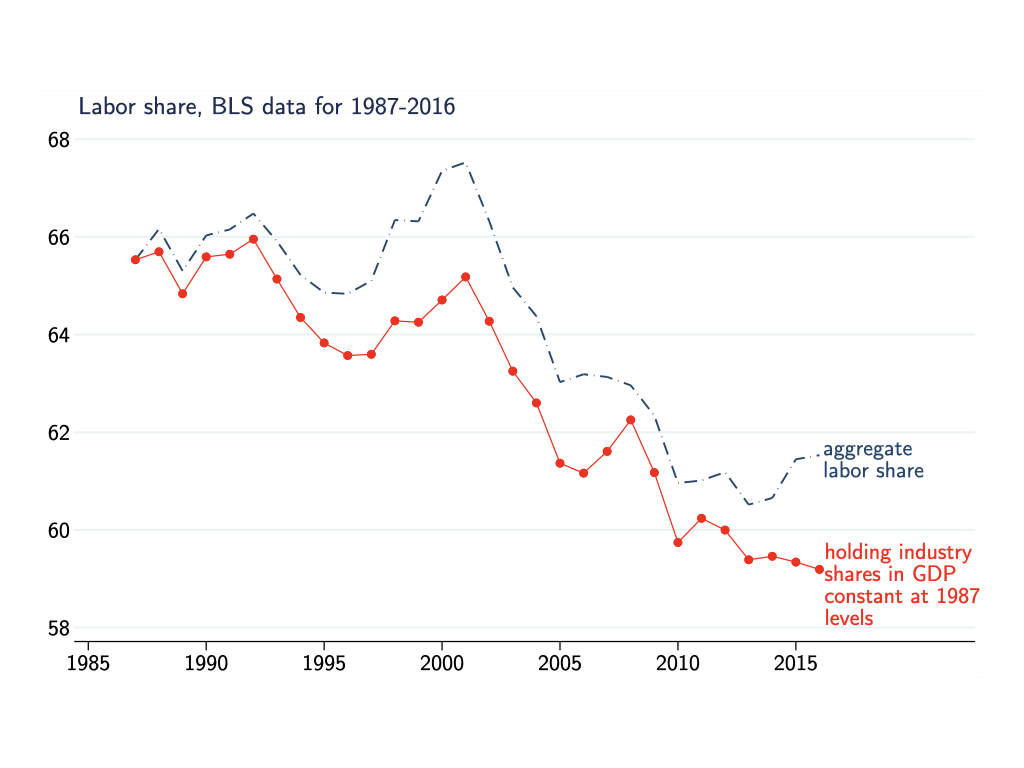
\includegraphics[height=8.5cm,width=\textwidth]{figureM2.png}
\end{figure}
\end{center}
\newpage

\newpage
\begin{center}
\begin{figure}
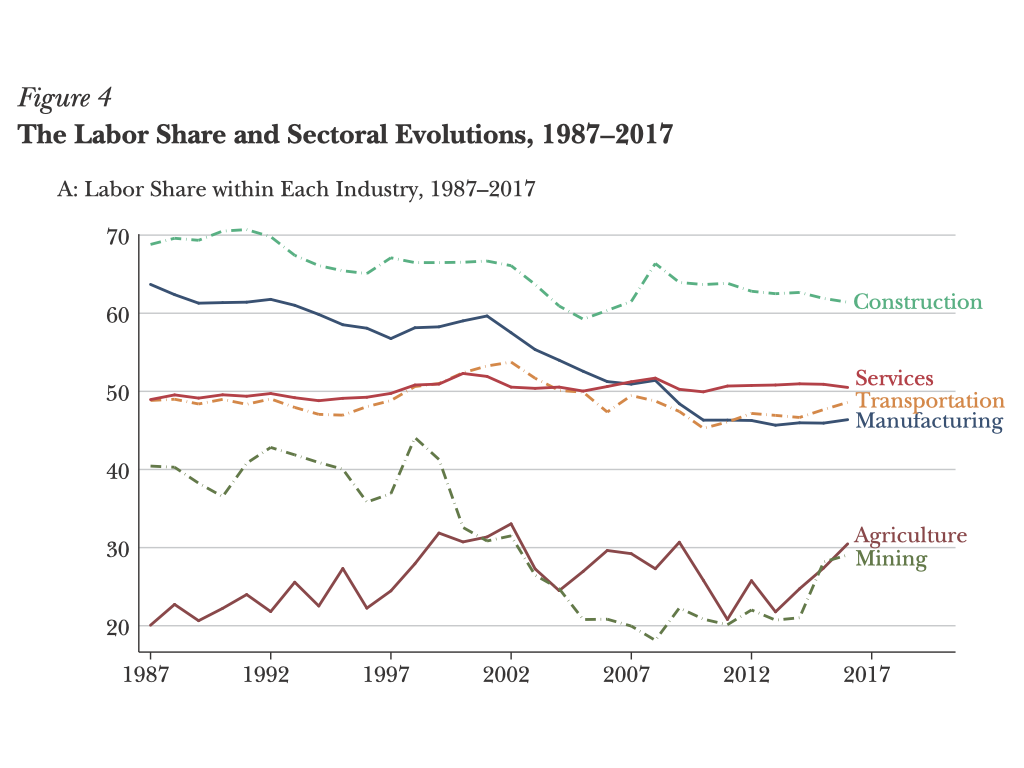
\includegraphics[height=8.5cm,width=\textwidth]{figureM3.png}
\end{figure}
\end{center}
\newpage

\begin{frame}{Motivation (Acemoglu \& Restrepo [18])}
\begin{itemize}
\item \textbf{2-factor CRS production functions assuming factor-augmenting technological change} pose important problems and puzzles. \medskip
\item \textbf{Capital-augmenting} technological change cannot explain declining wages for some workers or the recent fall in the labor share for realistic parameter values. \medskip
\item \textbf{Labor-augmenting} technological change cannot explain declining wages for realistic parameter values. \medskip
\item It could explain the recent fall in the labor share for realistic parameter values, but it is not very convincing conceptually.
\end{itemize}
\end{frame}

\begin{frame}{Table of Contents}
\begin{itemize}
\item[\textcolor{black}{1.}] \textcolor{black}{Conceptual Framework} \bigskip
\item[\textcolor{black}{2.}] \textcolor{black}{Sources of Labor Demand Growth in the United States} \bigskip
\item[\textcolor{black}{3.}] \textcolor{black}{Concluding Remarks}
\end{itemize}
\end{frame}

\section{1. Conceptual Framework}

\subsection{1.1 A task-based framework}

\begin{frame}{1. Conceptual Framework}
\begin{itemize}
\item[\textcolor{red}{1.1}] \textcolor{red}{A task-based framework} \bigskip
\item[\textcolor{gray}{1.2}] \textcolor{gray}{Types of technological change} \bigskip
\item[\textcolor{gray}{1.3}] \textcolor{gray}{Equilibrium} \bigskip
\item[\textcolor{gray}{1.4}] \textcolor{gray}{Technology and labor demand} \bigskip
\item[\textcolor{gray}{1.5}] \textcolor{gray}{Multi-sector economy} 
\end{itemize}
\end{frame}

\begin{frame}{Production technology}
\begin{itemize}
\item Static environment with a unique final good, $Y$. \medskip
\item $Y$ is produced with a continuum of tasks on the unit interval $[N-1,N]$ with $N$ an exogenous parameter. \medskip
\item CES technology mapping tasks into the final good:
\[
Y= \left[ \int_{N-1}^{N} y(z)^{\frac{\sigma-1}{\sigma}}dz \right]^{\frac{\sigma}{\sigma-1}} \tag{A1}  \label{eqA1}
\]
where $y(z)$ is output of task $z$ and $\sigma \geq 0 $ the elasticity of substitution between tasks. \medskip
\item The final good is the numeraire, $P \equiv 1$.
\end{itemize}
\end{frame}

\begin{frame}{The frontier of automation possibilities}
\begin{block}{Assumptions}
\begin{itemize}
\item Tasks $z \in [N-1,N]$ are ranked such that they become increasingly more difficult for machines to do. \medskip
\item Assume an exogenous threshold $I$ which is the frontier of automation possibilities. \medskip
\item All tasks $z \leq I$ can (and will) be automated, and all tasks $z > I $ can only be done by labor. \medskip
\item An increase in $I$ willl capture automation. 
\end{itemize}
\end{block}
\end{frame}

\begin{frame}{Supply of labor and capital to tasks}
\begin{itemize}
\item Task $z$ can be produced by labor, $l(z)$ or by capital, $k(z)$, according to:
\[
y(z) = 
\begin{cases}
A^{L} \gamma^{L}(z)l(z) + A^{K} \gamma^{K}(z)k(z) \text{ if } z \in [N-1,I]\\
A^{L} \gamma^{L}(z)l(z) \text{ if } z \in (I,N] 
\end{cases}
\]
where:
\begin{itemize}
\item $A^{L}, A^{K}$ are factor-augmenting technologies \medskip
\item $ \gamma^{L}(z), \gamma^{K}(z)$ are task productivity schedules \medskip
\item $ l(z), k(z)$ are the number of each factor allocated to task $z$
\end{itemize}
\end{itemize}
\end{frame}

\begin{frame}{Comparative advantage in task production}
\begin{block}{Assumption}
$ \gamma^{L}(z)/\gamma^{K}(z)$ is strictly increasing in $z$.
\end{block}
\begin{itemize}
\item This is an assumption about the \textit{relative} productivity of labor and capital in doing different tasks. \medskip
\item This assumption drives factor allocation across tasks based on comparative advantage (as in Roy [51]).\medskip
\item All tasks $z \in [N-1,I]$ will be done by capital and all tasks $z \in (I,N]$ will be done by labor. 
\end{itemize}
\end{frame}

\newpage
\begin{center}
\begin{figure}
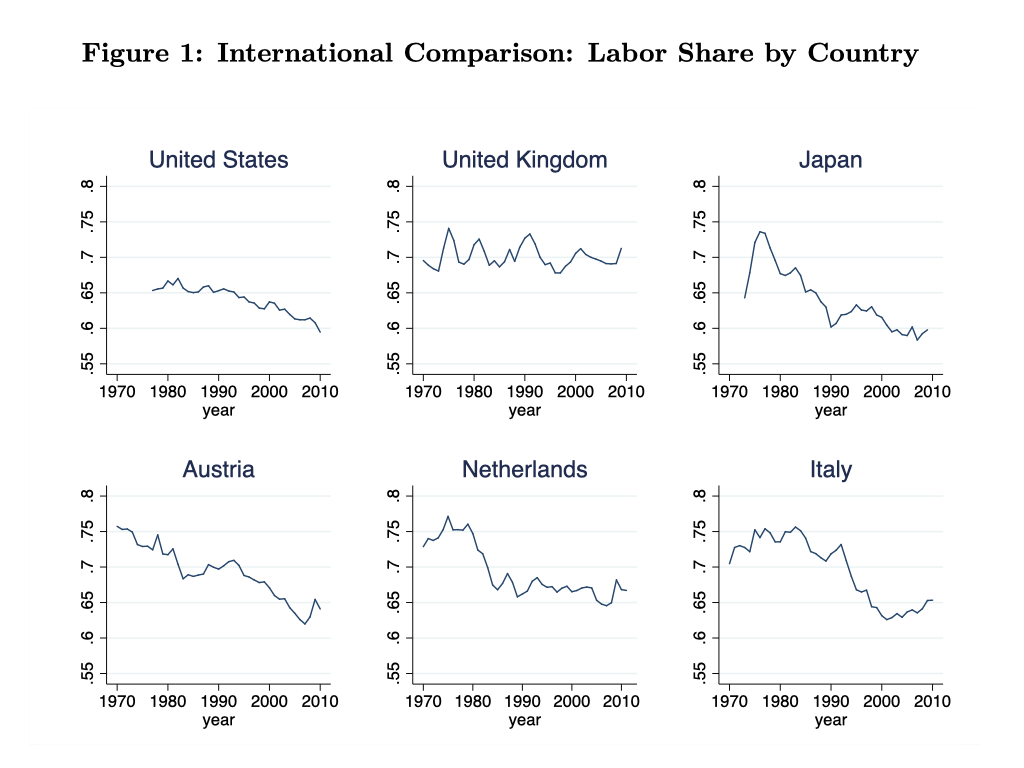
\includegraphics[height=7.5cm,width=\textwidth]{figure1a.png}
\\ Allocation of tasks to factors
\end{figure} 
\end{center}
\newpage

\begin{frame}{Clearing factor markets}
\begin{itemize}
\item Labor and capital are supplied inelastically by $L$ and $K$ respectively (this will no longer hold in section 1.5). \medskip
\item Labor markets clearing requires:
\[
\int_{N-1}^{N} l(z)dz = L \text{ and } \int_{N-1}^{N} k(z)dz = K
\]
\item In this environment, we can look at: \medskip
\begin{itemize}
\item Types of technological change (section 1.2) \medskip
\item Equilibrium (section 1.3) \medskip
\item Technology and labor demand (section 1.4) \medskip
\item Multi-sector economy (section 1.5)
\end{itemize}
\end{itemize}
\end{frame}

\subsection{1.2 Types of technological change}

\begin{frame}{1. Conceptual Framework}
\begin{itemize}
\item[\textcolor{gray}{1.1}] \textcolor{gray}{A task-based framework} \bigskip
\item[\textcolor{red}{1.2}] \textcolor{red}{Types of technological change} \bigskip
\item[\textcolor{gray}{1.3}] \textcolor{gray}{Equilibrium} \bigskip
\item[\textcolor{gray}{1.4}] \textcolor{gray}{Technology and labor demand} \bigskip
\item[\textcolor{gray}{1.5}] \textcolor{gray}{Multi-sector economy} 
\end{itemize}
\end{frame}

\newpage
\begin{center}
\begin{figure}
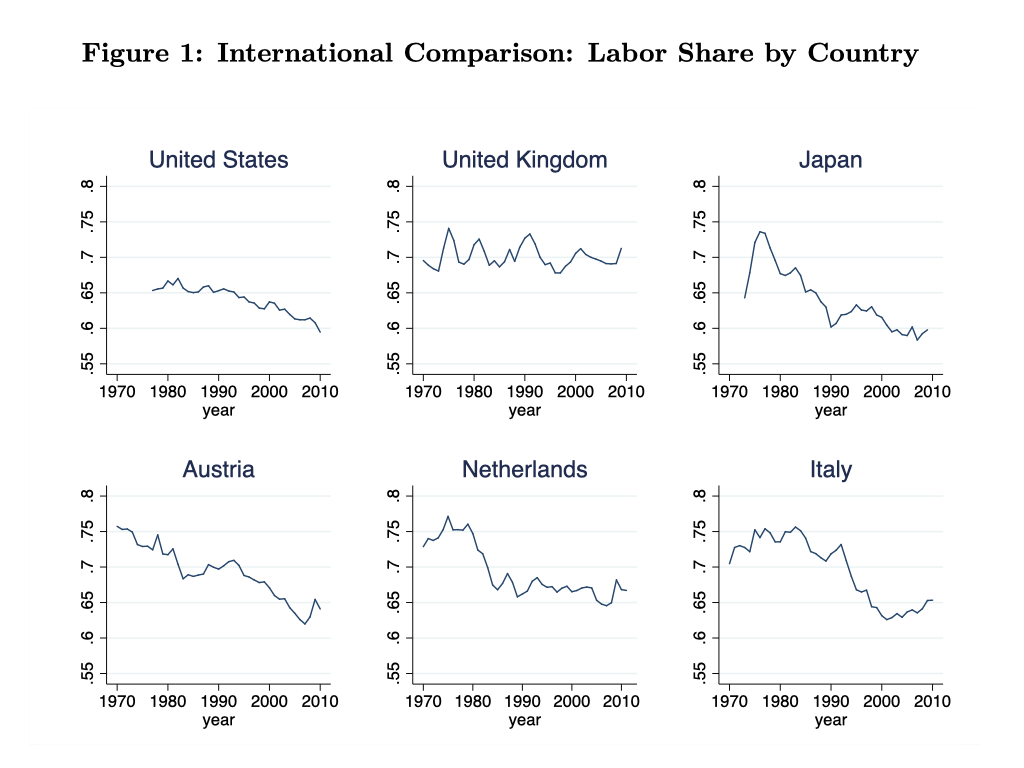
\includegraphics[height=7.5cm,width=\textwidth]{figure1a.png}
\\ Allocation of tasks to factors
\end{figure} 
\end{center}
\newpage

\begin{frame}{Types of technological change}
\begin{enumerate}
\item \textbf{Labor-augmenting technological change}: \\
$A^{L} \uparrow$ or $\gamma^{L}(z) \uparrow$ for all $z$\medskip
\item \textbf{Automation (at the extensive margin)}: \\
Automation possibility frontier $I \uparrow $ \medskip
\item \textbf{Deepening of automation (at the intensive margin)}: \\
$A^{K} \uparrow$ or $\gamma^{K}(z) \uparrow$ for all $z < I$ \medskip
\item \textbf{Creation of new labor-intensive tasks}: \\
$N \uparrow $ which increases the bounds of the unit interval of tasks ranked by labor's comparative advantage
\end{enumerate}
\end{frame}

\newpage
\begin{center}
\begin{figure}
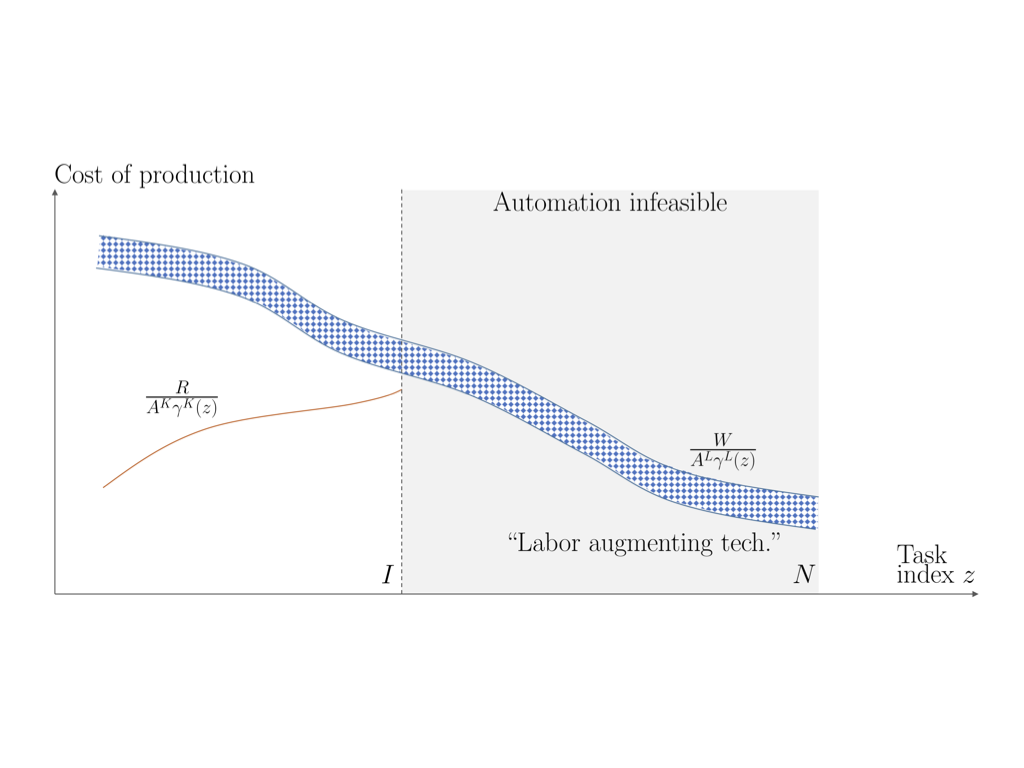
\includegraphics[height=7.5cm,width=\textwidth]{figure1c.png}
\\ 1. \textbf{Labor-augmenting technological change}: \\
$A^{L} \uparrow$ or $\gamma^{L}(z) \uparrow$ for all $z$
\end{figure} 
\end{center}
\newpage

\newpage
\begin{center}
\begin{figure}
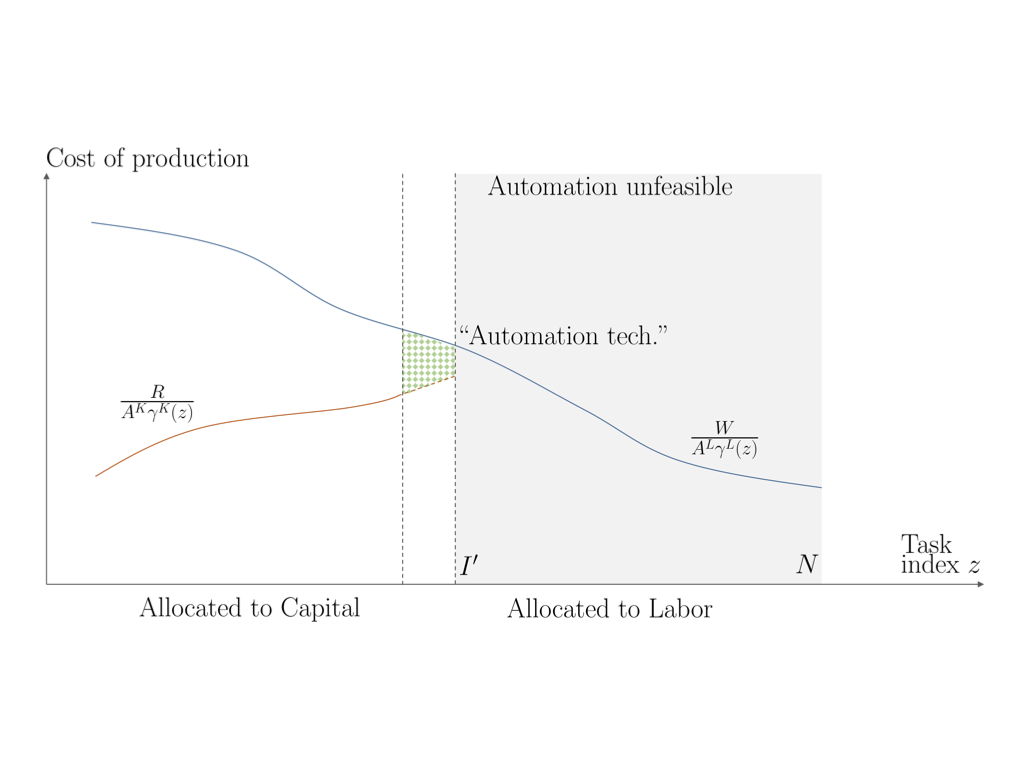
\includegraphics[height=7.5cm,width=\textwidth]{figure1d.png}
\\ 2. \textbf{Automation (at the extensive margin)}: \\
Automation possibility frontier $I \uparrow $
\end{figure} 
\end{center}
\newpage

\newpage
\begin{center}
\begin{figure}
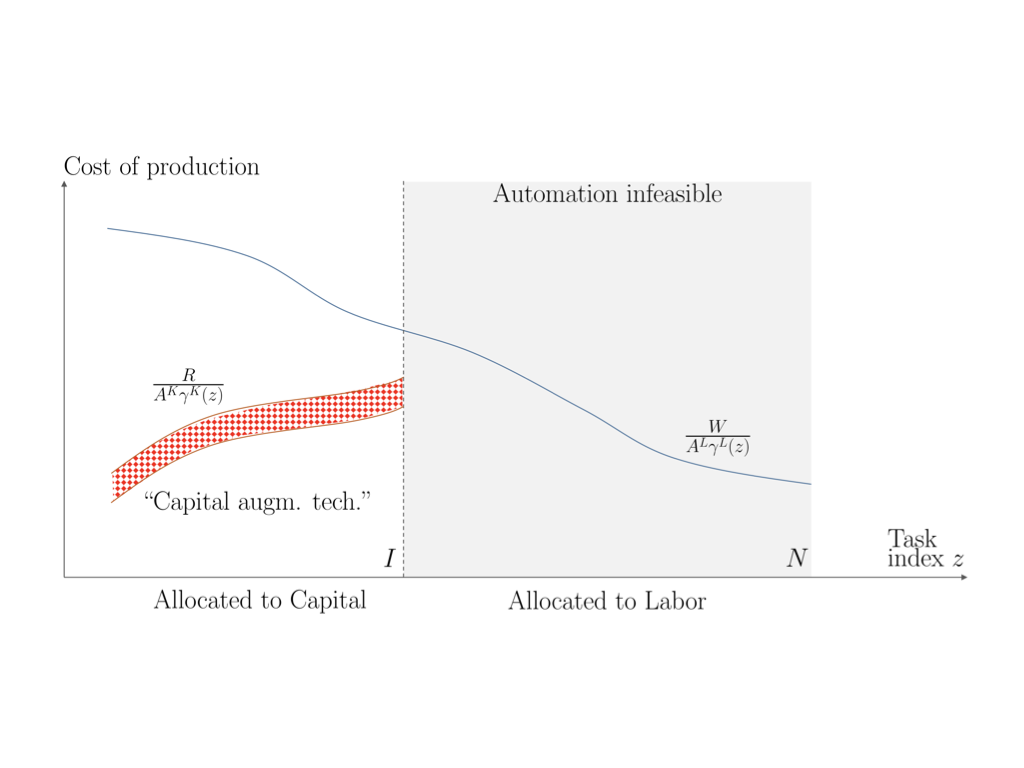
\includegraphics[height=7.5cm,width=\textwidth]{figure1b.png}
\\ 3. \textbf{Deepening of automation (at the intensive margin)}: \\
$A^{K} \uparrow$ or $\gamma^{K}(z) \uparrow$ for all $z < I$
\end{figure} 
\end{center}
\newpage

\newpage
\begin{center}
\begin{figure}
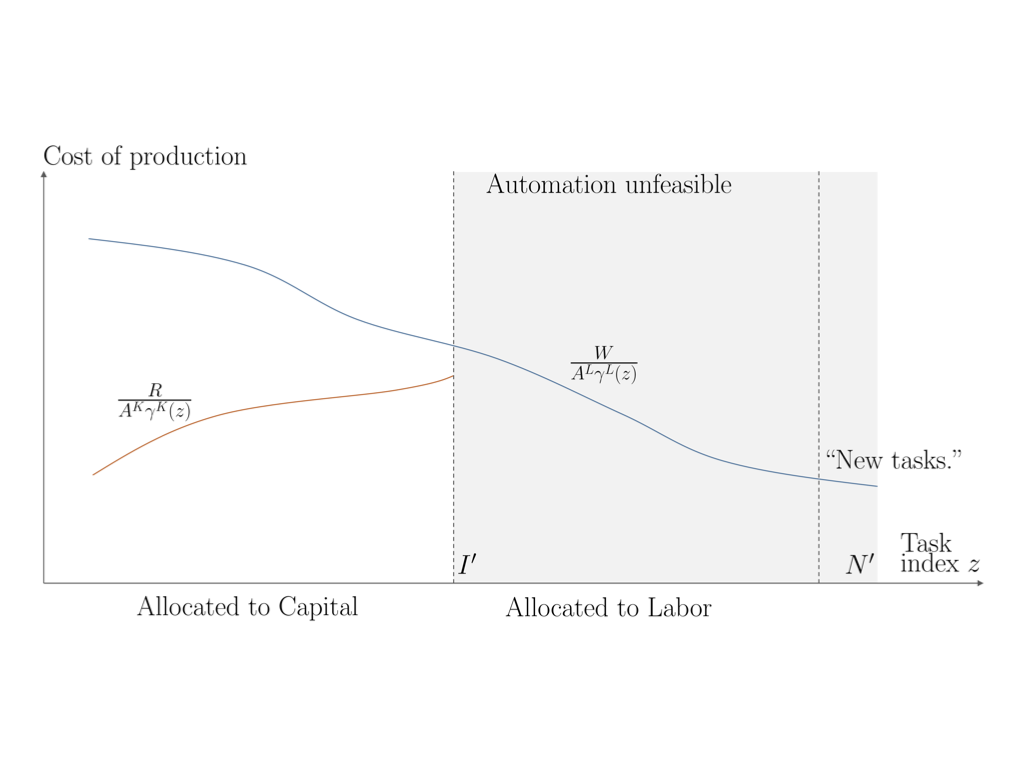
\includegraphics[height=7cm,width=\textwidth]{figure1e.png}
\\ 4. \textbf{Creation of new labor-intensive tasks}: \\
$N \uparrow $ which increases the bounds of the unit interval of tasks ranked by labor's comparative advantage
\end{figure} 
\end{center}
\newpage

\subsection{1.3 Equilibrium}

\begin{frame}{1. Conceptual Framework}
\begin{itemize}
\item[\textcolor{gray}{1.1}] \textcolor{gray}{A task-based framework} \bigskip
\item[\textcolor{gray}{1.2}] \textcolor{gray}{Types of technological change} \bigskip
\item[\textcolor{red}{1.3}] \textcolor{red}{Equilibrium} \bigskip
\item[\textcolor{gray}{1.4}] \textcolor{gray}{Technology and labor demand} \bigskip
\item[\textcolor{gray}{1.5}] \textcolor{gray}{Multi-sector economy} 
\end{itemize}
\end{frame}

\newpage
\begin{center}
\begin{figure}
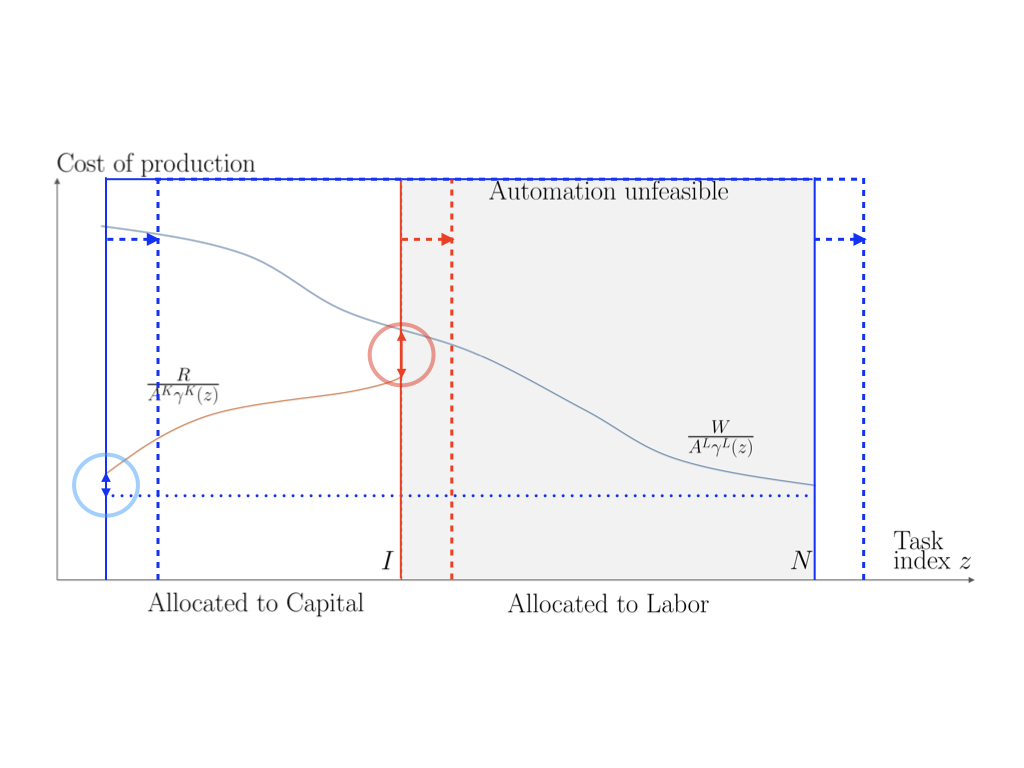
\includegraphics[height=7.5cm,width=\textwidth]{figure1f.png}
\\ Efficiencies at marginal tasks: equilibrium assumptions
\end{figure} 
\end{center}
\newpage

\begin{frame}{Efficiencies at marginal tasks: equilibrium assumptions}
\begin{itemize}
\item Denote the equilibrium wage rate by $W$ and rental rate by $R$. \medskip
\item Further assume that in any equilibrium:
\[
\color{red} \frac{A^{L}\gamma^{L}(I)}{A^{K}\gamma^{K}(I)} < \color{black} \frac{W}{R} \color{blue} < \frac{A^{L}\gamma^{L}(N)}{A^{K}\gamma^{K}(N-1)} \color{black} \tag{A7} \label{eqA7}
\]
\item First inequality implies that all tasks $z \in [N-1,I]$ will be produced by capital and that an increase in $I$ increases $Y$. \medskip
\item Second inequality implies that an increase in $N$ increases $Y$. \medskip
\item We return to these equilibrium assumptions below. 
\end{itemize}
\end{frame}

\begin{frame}{Task demands}
\begin{itemize}
\item CES technology mapping tasks into the final good:
\[
Y= \left[ \int_{N-1}^{N} y(z)^{\frac{\sigma-1}{\sigma}}dz \right]^{\frac{\sigma}{\sigma-1}} \tag{A1}  \label{eqA1}
\]
\item Gives demand for task $z$:
\[
y(z) = \frac{Y}{p(z)^{\sigma}}
\]
\item With the price of task $z$, $p(z)$, given by:
\[
p(z) = 
\begin{cases}
\frac{R}{A^{K} \gamma^{K}(z)} \text{ if } z \in [N-1,I] \\
\frac{W}{A^{L} \gamma^{L}(z)} \text{ if } z \in (I,N] 
\end{cases}
\]
\end{itemize}
\end{frame}

\begin{frame}{Factor demands in tasks}
\begin{itemize}
\item Using that $y(z) = A^{K} \gamma^{K}(z)k(z)$ for $z \in [N-1,I]$:
\[
k(z)=
\begin{cases}
\frac{Y}{A^{K}\gamma^{K}(z)} \left[ \frac{R}{A^{K}\gamma^{K}(z)} \right]^{- \sigma} \text{ if } z \in [N-1,I] \\
0 \text{ if } z \in (I,N]
\end{cases}
\]
which gives demand for capital in each task $z$. \medskip
\item Using that $y(z) = A^{L} \gamma^{L}(z)l(z)$ for $z \in (I,N]$:
\[
l(z)=
\begin{cases}
0 \text{ if } z \in [N-1,I] \\
\frac{Y}{A^{L}\gamma^{L}(z)} \left[ \frac{W}{A^{L}\gamma^{L}(z)} \right]^{- \sigma}  \text{ if } z \in (I,N]
\end{cases}
\]
which gives labor demand in each task $z$.
\end{itemize}
\end{frame}

\begin{frame}{Aggregate demand for labor and equilibrium wage}
\begin{itemize}
\item The market clearing condition for labor is:
\[
L = \int_{N-1}^{N} l(z)dz =  \int_{I}^{N} \frac{Y}{A^{L}\gamma^{L}(z)} \left[ \frac{W}{A^{L}\gamma^{L}(z)} \right]^{- \sigma} dz
\]
\item Re-arranging terms gives the equilibrium wage:
\begin{tcolorbox}
\[
W = \left[ \frac{Y}{L} \int_{I}^{N} [A^{L}\gamma^{L}(z)]^{\sigma-1} dz \right]^{\frac{1}{\sigma}}
\]
\end{tcolorbox}
\item \textbf{Sneak preview}: Automation (i.e. an increase in $I$) results in a negative displacement and a positive productivity effect. New tasks (i.e. an increase in $N$) results in positive reinstatement and productivity effects.  
\end{itemize}
\end{frame}

\begin{frame}{Aggregate demand for capital and equilibrium rental rate}
\begin{itemize}
\item The market clearing condition for capital is:
\[
K = \int_{N-1}^{N} k(z)dz =  \int_{N-1}^{I} \frac{Y}{A^{K}\gamma^{K}(z)} \left[ \frac{R}{A^{K}\gamma^{K}(z)} \right]^{- \sigma} dz
\]
\item Re-arranging terms gives the equilibrium rental rate:
\begin{tcolorbox}
\[
R = \left[ \frac{Y}{K} \int_{N-1}^{I} [A^{K}\gamma^{K}(z)]^{\sigma-1} dz \right]^{\frac{1}{\sigma}}
\]
\end{tcolorbox}
\item We can use expressions for $W$ and $R$ above in $P=MC$ to derive an expression for aggregate output $Y$ in equilibrium.
\end{itemize}
\end{frame}

\begin{frame}{The aggregate price index in equilibrium}
\begin{itemize}
\item Profit maximization implies that price equals marginal costs:
\[
P = \left[ \int_{N-1}^{N} p(z)^{1-\sigma} dz \right]^{\frac{1}{1- \sigma}}  \equiv 1
\]
\item This implies that:
\[
\int_{N-1}^{N} p(z)^{1-\sigma} dz = 1
\]
\item Using the expressions for $p(z)$:
 \[
\int_{N-1}^{I} \left[\frac{R}{A^{K} \gamma^{K}(z)} \right]^{1-\sigma} dz + \int_{I}^{N} \left[ \frac{W}{A^{L} \gamma^{L}(z)} \right]^{1-\sigma} dz = 1
\]
\end{itemize}
\end{frame}

\begin{frame}{Aggregate output in equilibrium}
\begin{itemize}
\item Using equilibrium expressions for $W$ and $R$ and rearranging terms gives:
\begin{align*}
Y^{\frac{\sigma-1}{\sigma}} = & \left[ \int_{N-1}^{I} \gamma^{K}(z)^{\sigma-1} dz \right]^{\frac{1}{\sigma}} [A^{K}K]^{\frac{\sigma -1}{\sigma}} \\
& + \left[ \int_{I}^{N} \gamma^{L}(z)^{\sigma-1} dz \right]^{\frac{1}{\sigma}} [A^{L}L]^{\frac{\sigma -1}{\sigma}} \tag{A2} \label{eqA2}
\end{align*}
\item We can define $\Pi(I,N)$ and $\Gamma(I,N)$ such that:
\[
Y= \Pi(I,N) \left[ [1- \Gamma(I,N)]^{\frac{1}{\sigma}} [A^{K}K]^{\frac{\sigma -1}{\sigma}} + \Gamma(I,N)^{\frac{1}{\sigma}} [A^{L}L]^{\frac{\sigma -1}{\sigma}} \right]^{\frac{\sigma}{\sigma-1}} 
\]
\end{itemize}
\end{frame}

\begin{frame}{A microfounded aggregate CES production function}
\[
Y= \color{orange} \Pi(I,N) \color{black} \left[ \color{orange} [1- \Gamma(I,N)] \color{black} ^{\frac{1}{\sigma}} [ \color{cyan}A^{K} \color{black}K]^{\frac{\sigma -1}{\sigma}} + \color{orange} \Gamma(I,N)\color{black}^{\frac{1}{\sigma}} [\color{cyan}A^{L}\color{black}L]^{\frac{\sigma -1}{\sigma}} \right]^{\frac{\sigma}{\sigma-1}} 
\]
with \textcolor{orange}{\textbf{task content of production}} given by:
\[
\color{orange} \Pi(I,N) \equiv \left[ \int_{N-1}^{I} \gamma^{K}(z)^{\sigma-1} dz + \int_{I}^{N} \gamma^{L}(z)^{\sigma-1} dz \right]^{\frac{1}{\sigma - 1}} \color{black} \tag{A4} \label{eqA4}
\]
\[
\color{orange} \Gamma(I,N) \equiv \left[ \int_{I}^{N} \gamma^{L}(z)^{\sigma-1} dz \right] \Pi(I,N)^{1-\sigma} \color{black} \tag{A3} \label{eqA3}
\]
with \textcolor{cyan}{\textbf{factor-augmenting}} technological change given by:
\[
\color{cyan} A^{K} \color{black} \uparrow \text{ if capital-augmenting and } \color{cyan} A^{L} \color{black} \uparrow \text{ if labor-augmenting}
\]
\end{frame}

\begin{frame}{Microfounded aggregate production functions}
\begin{itemize}
\item This can be summarized by:
\begin{tcolorbox}
\[
Y = \color{orange} \Pi(I,N) \color{black}F(\color{cyan}A^{K} \color{black}K,\color{cyan}A^{L}\color{black}L; \color{orange}\Gamma(I,N) \color{black}) 
\]
where \textbf{technological change} works through:
\begin{enumerate}
\item \textcolor{orange}{\textbf{Changing task content}} through a TFP-term $\color{orange}\Pi(I,N)$ and the distribution parameter $\color{orange}\Gamma(I,N) \in (0,1)$
\item \textcolor{cyan}{\textbf{Factor-augmenting}} through $\color{cyan} A^{K} \color{black} \uparrow$ or $\color{cyan} A^{L} \color{black} \uparrow$
\end{enumerate}
\end{tcolorbox}
\item We assumed a CES task production function. \medskip
\item We could also assume a Cobb-Douglas task production function (as in Acemoglu \& Restrepo[19]).
\end{itemize}
\end{frame}

\begin{frame}{A microfounded aggregate Cobb-Douglas production function}
\[
Y = \color{orange} \Pi(I,N) \color{black} \left[ \frac{\color{cyan}A^{K} \color{black}K}{\color{orange}1-\Gamma(I,N)} \color{black}\right]^{\color{orange} 1-\Gamma(I,N)} \color{black} \left[ \frac{\color{cyan}A^{L} \color{black}L}{\color{orange}\Gamma(I,N)} \color{black} \right]^{\color{orange} \Gamma(I,N)} 
\]
with \textcolor{orange}{\textbf{task content of production}} given by:
\[
\color{orange} \Pi(I,N) \equiv \exp \left[ \int_{N-1}^{I} \ln(\gamma^{K}(z))dz + \int_{I}^{N} \ln(\gamma^{L}(z))dz \right] 
\]
\[
\color{orange} \Gamma(I,N) \equiv N-I \color{black} \text{ and } \color{orange} 1 - \Gamma(I,N)=I - N + 1 \color{black} 
\]
with \textcolor{cyan}{\textbf{factor-augmenting}} technological change given by:
\[
\color{cyan} A^{K} \color{black} \uparrow \text{ if capital-augmenting and } \color{cyan} A^{L} \color{black} \uparrow \text{ if labor-augmenting}
\]
\end{frame}

\begin{frame}{Microfounded aggregate production functions}
\begin{itemize}
\item We have derived an aggregate production function where differential technological change works through different channels.
\item In particular, technological progress changes the distribution parameter and the Hicks-neutral TFP term. \medskip
\item Task models provide microfoundations for changes in the distribution parameter and TFP due to technical progress. \medskip
\item It assumes that automation of labor tasks and the creation of new labor-intensive tasks results in a reallocation of factors across tasks and overall productivity effects. 
\end{itemize}
\end{frame}

\begin{frame}{Factor shares}
\begin{itemize}
\item The labor share is given by $s_{L}=WL/Y$. \medskip
\item Using the expressions for $W$ and $Y$ above gives:
\begin{tcolorbox}
\[
s_{L} = \left[ 1+ [\frac{1-\Gamma(I,N)}{\Gamma(I,N)}]^{\frac{1}{\sigma}} [\frac{A^{K}K}{A^{L}L}]^{\frac{\sigma-1}{\sigma}} \right]^{-1} \tag{A5} \label{eqA5}
\]
\end{tcolorbox}
\item Using the expression for $W/R$ in equilibrium gives:
\begin{tcolorbox}
\[
s_{L} = \left[ 1+ [\frac{1-\Gamma(I,N)}{\Gamma(I,N)}] [\frac{A^{L}}{W} \frac{R}{A^{K}}]^{1-\sigma} \right]^{-1} \tag{A4} \label{eqA4}
\]
\end{tcolorbox}
\item Given constant returns to scale, $s_{K}=1-s_{L}$.
\end{itemize}
\end{frame}

\newpage
\begin{center}
\begin{figure}
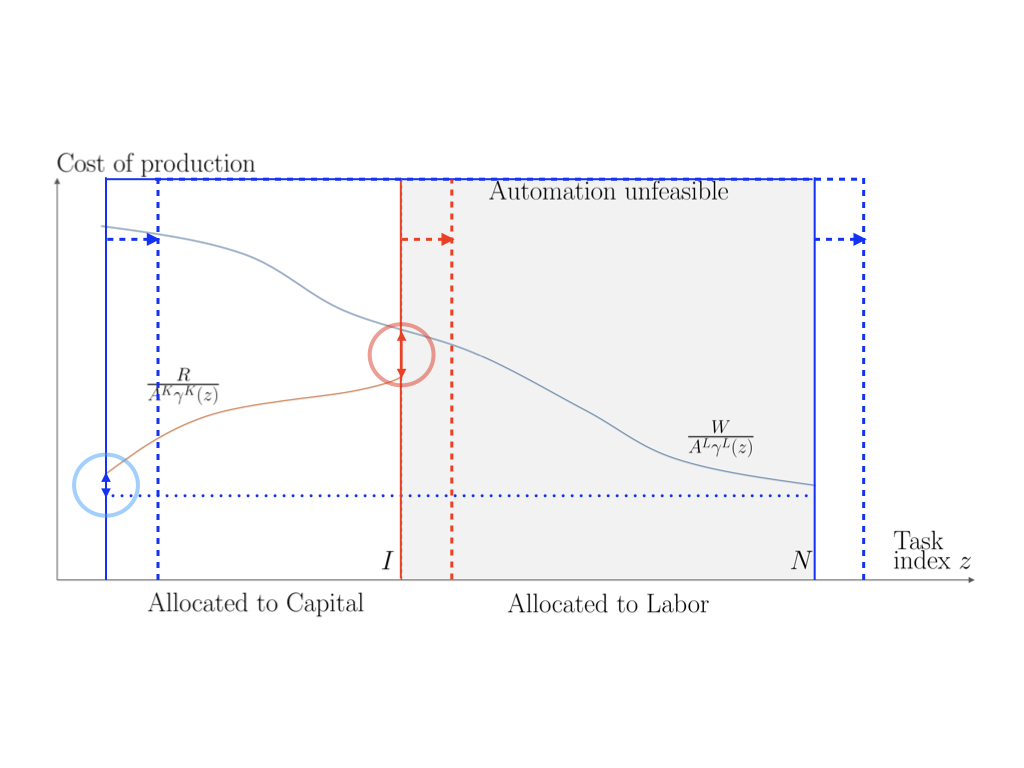
\includegraphics[height=7.5cm,width=\textwidth]{figure1f.png}
\\ Efficiencies at marginal tasks: equilibrium assumptions
\end{figure} 
\end{center}
\newpage

\begin{frame}{Equilibrium assumptions revisited}
\begin{itemize}
\item To ensure that technological progress raises productivity, we assumed that:
\[
\color{red} \frac{A^{L}\gamma^{L}(I)}{A^{K}\gamma^{K}(I)} < \color{black} \frac{W}{R} \color{blue} < \frac{A^{L}\gamma^{L}(N)}{A^{K}\gamma^{K}(N-1)} \color{black} \tag{A7}
\] \label{eqA7}
\item Using the expression for $W/R$, this is equivalent to assuming:
\[
\color{black} \frac{K}{L} > \color{red} \frac{1-\Gamma(I,N)}{\Gamma(I,N)} \left[ \frac{A^{L}}{A^{K}} \frac{\gamma^{L}(I)}{\gamma^{K}(I)} \right]^{\sigma}
\]
\[
\color{black} \frac{K}{L} < \color{blue} \frac{1-\Gamma(I,N)}{\Gamma(I,N)} \left[ \frac{A^{L}}{A^{K}} \frac{\gamma^{L}(N)}{\gamma^{K}(N-1)} \right]^{\sigma} \color{black} \tag{A6}
\]
\end{itemize}
\end{frame}

\subsection{1.4 Technology and labor demand}

\begin{frame}{1. Conceptual Framework}
\begin{itemize}
\item[\textcolor{gray}{1.1}] \textcolor{gray}{A task-based framework} \bigskip
\item[\textcolor{gray}{1.2}] \textcolor{gray}{Types of technological change} \bigskip
\item[\textcolor{gray}{1.3}] \textcolor{gray}{Equilibrium} \bigskip
\item[\textcolor{red}{1.4}] \textcolor{red}{Technology and labor demand} \bigskip
\item[\textcolor{gray}{1.5}] \textcolor{gray}{Multi-sector economy} 
\end{itemize}
\end{frame}

\begin{frame}{The impact of automation on factor demands}
\begin{itemize}
\item Using the expression for $W$, the impact of automation on labor demand is given by:
\[
\frac{d \ln (W)}{dI} = \underbrace{\frac{1}{\sigma} \frac{d \ln (Y/L)}{dI}}_{\text{Productivity effect} >0} \underbrace{- \frac{1}{\sigma} \frac{\gamma_{L}(I)^{\sigma-1}}{\int_{I}^{N} \gamma^{L}(z)^{\sigma - 1} dz }}_{\text{Displacement effect}<0}
\]
\item Using the expression for $R$, the impact of automation on capital demand is given by:
\[
\frac{d \ln (R)}{dI} = \underbrace{\frac{1}{\sigma} \frac{d \ln (Y/K)}{dI}}_{\text{Productivity effect} >0} \underbrace{+ \frac{1}{\sigma} \frac{\gamma_{K}(I)^{\sigma-1}}{\int_{N-1}^{I} \gamma^{K}(z)^{\sigma - 1} dz }}_{\text{Expansion effect}>0}
\]
\end{itemize}
\end{frame}

\begin{frame}{The impact of new tasks on factor demands}
\begin{itemize}
\item Using the expression for $W$, the impact of new tasks on labor demand is given by:
\[
\frac{d \ln (W)}{dN} = \underbrace{\frac{1}{\sigma} \frac{d \ln (Y/L)}{dN}}_{\text{Productivity effect} >0} \underbrace{+ \frac{1}{\sigma} \frac{\gamma_{L}(N)^{\sigma-1}}{\int_{I}^{N} \gamma^{L}(z)^{\sigma - 1} dz }}_{\text{Reinstatement effect}>0}
\]
\item Using the expression for $R$, the impact of new tasks on capital demand is given by:
\[
\frac{d \ln (R)}{dN} = \underbrace{\frac{1}{\sigma} \frac{d \ln (Y/K)}{dN}}_{\text{Productivity effect} >0} \underbrace{- \frac{1}{\sigma} \frac{\gamma_{K}(N-1)^{\sigma-1}}{\int_{N-1}^{I} \gamma^{K}(z)^{\sigma - 1} dz }}_{\text{Destruction effect}<0}
\]
\end{itemize}
\end{frame}

\begin{frame}{The productivity effects from automation and new tasks}
\begin{itemize}
\item Using the equation (A2), the productivity effect from automation is given by:
\[
\frac{d \ln (Y) }{dI} = \frac{1}{\sigma -1} \left[ \left[ \frac{R}{A^{K}\gamma^{K}(I)} \right] ^{1- \sigma} - \left[ \frac{W}{A^{L} \gamma^{L}(I)} \right]^{1- \sigma} \right] > 0
\]
\item Using the equation (A2), the productivity effect from new tasks is given by:
\[
\frac{d \ln (Y) }{dN} = \frac{1}{\sigma -1} \left[ \left[ \frac{W}{A^{L} \gamma^{L}(N)} \right]^{1- \sigma} - \left[ \frac{R}{A^{K}\gamma^{K}(N-1)} \right]^{1- \sigma} \right] > 0
\]
\end{itemize}
\end{frame}

\begin{frame}{An alternative way to write changes in labor demand}
\begin{itemize}
\item The labor share is given by:
\[
s_{L} = \frac{WL}{Y} =  \left[ 1+ [\frac{1-\Gamma(I,N)}{\Gamma(I,N)}]^{\frac{1}{\sigma}} [\frac{A^{K}K}{A^{L}L}]^{\frac{\sigma-1}{\sigma}} \right]^{-1} \tag{A5}
\]
\item Alternative ways to write the change in labor demand due to automation and new tasks therefore are:
\[
\frac{d \ln (W)}{dI} = \frac{d \ln (Y/L)}{dI} + \frac{d \ln (s_{L})}{dI} \tag{A8} \label{eqA8}
\]
\[
\frac{d \ln (W)}{dN} = \frac{d \ln (Y/L)}{dN} + \frac{d \ln (s_{L})}{dN} 
\]
\item To rewrite (A8), totally differentiate $ \ln (s_{L})$ using (A5).
\end{itemize}
\end{frame}

\begin{frame}{Differentiating the labor share}
\begin{itemize}
\item Totally differentiating the labor share using (A5) gives:
\[
d \ln (s_{L}) = \frac{1}{\sigma} \frac{1-s_{L}}{1- \Gamma} d \ln (\Gamma(I,N)) - \frac{\sigma -1}{\sigma} [1-s_{L}] d \ln (\frac{A^{K}}{A^{L}}\frac{K}{L})
\]
\item The first term captures the impact of automation and new tasks, and the second term the impact of factor-augmenting changes (or changes in $K$ and $L$). \medskip
\item Alternatively, totally differentiating (A4) instead of (A5) gives:
\[
d \ln (s_{L}) = \frac{1-s_{L}}{1- \Gamma} d \ln (\Gamma(I,N)) - [1- \sigma] [1-s_{L}] d \ln (\frac{A^{L}}{A^{K}}\frac{R}{W})
\]
\end{itemize}
\end{frame}

\begin{frame}{The impact of automation and new tasks on labor demand}
\begin{itemize}
\item The impact of automation on labor demand is given by:
\[
\frac{d \ln (W)}{dI} = \underbrace{\frac{d \ln (Y/L)}{dI}}_{\text{Productivity effect} >0} + \underbrace{\frac{1}{\sigma} \frac{1-s_{L}}{1- \Gamma} \frac{d \ln (\Gamma(I,N))}{dI}}_{\text{Displacement effect}<0}
\]
with $d \ln (\Gamma) / dI <0$ from equation (A3).
\item The impact of new tasks on labor demand is given by:
\[
\frac{d \ln (W)}{dN} = \underbrace{\frac{d \ln (Y/L)}{dN}}_{\text{Productivity effect}>0} + \underbrace{\frac{1}{\sigma} \frac{1-s_{L}}{1- \Gamma} \frac{d \ln (\Gamma(I,N))}{dN}}_{\text{Reinstatement effect}>0}
\]
with $d \ln (\Gamma) / dN >0$ from equation (A3).
\end{itemize}
\end{frame}

\begin{frame}{Automation, new tasks, and the labor share}
\begin{itemize}
\item Assuming only automation and new tasks, we have that:
\[
d \ln (s_{L}) = \frac{1}{\sigma} \frac{1-s_{L}}{1- \Gamma} \left[ \underbrace{\frac{d \ln (\Gamma(I,N))}{dI}}_{<0} + \underbrace{\frac{d \ln (\Gamma(I,N))}{dN}}_{>0} \right]
\]
\item Automation decreases the labor share (despite productivity effects) whereas the creation of new labor-intensive tasks increases the labor share. \medskip
\item A constant labor share suggests that both forces balance each other out, a falling labor share suggests that automation is more important than the creation of new labor intensive tasks.
\end{itemize}
\end{frame}

\begin{frame}{Factor-augmenting technological progress and labor demand}
\begin{itemize}
\item The impact of labor-augmenting progress is given by:
\begin{align*}
\frac{d \ln (W) }{d \ln (A^{L})} = & \text{ \hspace{0.2cm}} s_{L} \text{ \hspace{2.5cm}(Productivity effect)} \\
& + \frac{\sigma - 1}{ \sigma} [1-s_{L}] \text{ \hspace{0.5cm}(Substitution effect)}
\end{align*}
\item The impact of capital-augmenting progress is given by:
\begin{align*}
\frac{d \ln (W) }{d \ln (A^{K})} = & \text{ \hspace{0.2cm}} [1- s_{L}] \text{ \hspace{1.8cm}(Productivity effect)} \\
& + \frac{1- \sigma}{ \sigma} [1-s_{L}] \text{ \hspace{0.7cm}(Substitution effect)}
\end{align*}
\end{itemize}
\end{frame}

\subsection{1.5 Multi-sector economy}

\begin{frame}{1. Conceptual Framework}
\begin{itemize}
\item[\textcolor{gray}{1.1}] \textcolor{gray}{A task-based framework} \bigskip
\item[\textcolor{gray}{1.2}] \textcolor{gray}{Types of technological change} \bigskip
\item[\textcolor{gray}{1.3}] \textcolor{gray}{Equilibrium} \bigskip
\item[\textcolor{gray}{1.4}] \textcolor{gray}{Technology and labor demand} \bigskip
\item[\textcolor{red}{1.5}] \textcolor{red}{Multi-sector economy} 
\end{itemize}
\end{frame}

\begin{frame}{A multi-sector economy}
The economy-wide wage bill, $WL$, is given by:
\[
WL = \sum_{i} W_{i} L_{i} = \sum_{i} P_{i} Y_{i} s_{i}^{L} = \sum_{i } Y \chi_{i} s_{i}^{L}
\]
with $i$ sector $i$ and where 
\[
s_{i}^{L} = \frac{W_{i}L_{i}}{P_{i}Y_{i}} \text{ \hspace{1cm} the labor share in sector i \hspace{0.9cm}}
\]
\[
Y = \sum_{i}  P_{i} Y_{i} \text{ \hspace{0.9cm} economy-wide value added \hspace{0.7cm}}
\]
\[
\chi_{i} = \frac{P_{i}Y_{i}}{Y} \text{ \hspace{0.7cm} sector i's share in total value added}
\]
\end{frame}

\begin{frame}{Decomposing changes in the aggregate wage bill}
\begin{itemize}
\item Totally differentiating the economy-wide wage bill gives:
\[
d(WL) = \sum_{i} dY \chi_{i} s_{i}^{L} + \sum_{i} Y d\chi_{i} s_{i}^{L} + \sum_{i} Y \chi_{i} ds_{i}^{L}
\]
\item Dividing both sides by $WL$ gives:
\[
d \ln (WL) = d \ln (Y) + \sum_{i} \frac{s_{i}^{L}}{s^{L}} d \chi_{i} + \sum_{i} l_{i} d \ln (s_{i}^{L})
\]
with $s^{L}$ the aggregate labor share and 
\[
l_{i} \equiv \frac{W_{i}L_{i}}{WL} \text{   such that   } \sum_{i} l_{i} = 1
\]
\end{itemize}
\end{frame}

\begin{frame}{Decomposing changes in the aggregate wage bill}
\begin{itemize}
\item Using the expression for $d \ln (s_{i}^{L})$ above gives \underline{equation (A9)}:
\begin{align*}
d \ln (WL) =  & d \ln (Y) \text{ \hspace{3.8cm} (Productivity effect)} \\
& +  \sum_{i} \frac{s_{i}^{L}}{s^{L}} d \chi_{i} \text{ \hspace{3cm} (Composition effect)} \\
& + \sum_{i} l_{i} [1- \sigma][1-s_{i}^{L}]d \ln (\frac{A_{i}^{K}W_{i}}{A_{i}^{L}R_{i}}) \text{\hspace{0.5cm}  (Subst. effect)} \\
& + \sum_{i} l_{i} \frac{1-s_{i}^{L}}{1- \Gamma_{i}} d \ln \Gamma_{i} \text{ \hspace{1.4cm} (Change task content)}
\end{align*}
\item The last two terms capture changes in $d \ln (s_{i}^{L})$ due to changes in relative effective factor prices (Substitution effect) and $dI$ or $dN$ (Change task content).
\end{itemize}
\end{frame}

\begin{frame}{Displacement versus reinstatement effects}
\begin{itemize}
\item The change in task content due to $dI$ or $dN$ was given by:
\[
 \sum_{i} l_{i} \frac{1-s_{i}^{L}}{1- \Gamma_{i}} d \ln \Gamma_{i}
\]
which is measured as a residual using equation (A9). \medskip
\item It consists of displacement and reinstatement effect given by:
\[
\text{Displacement}= \sum_{i} l_{i} \min \left[ 0, \frac{1-s_{i}^{L}}{1- \Gamma_{i}} d \ln \Gamma_{i} \right] \tag{A14a} \label{eq14a}
\]
\[
\text{Reinstatement}= \sum_{i} l_{i} \max \left[ 0, \frac{1-s_{i}^{L}}{1- \Gamma_{i}} d \ln \Gamma_{i} \right] \tag{A14b} \label{eq14b}
\]
\end{itemize}
\end{frame}

\section{2. Sources of Labor Demand Growth in the United States}

\begin{frame}{Data}
\begin{itemize}
\item \underline{Data for 1987-2017}: BEA GDP by Industry Accounts for measures of $P_{i}Y_{i}$ and $W_{i}L_{i}$, and BLS Multifactor Productivity Tables for measures of $W_{i}$ and $R_{i}$ for 61 private NAICS industries. \medskip
\item \underline{Data for 1947-1987}: BEA GDP by Industry Accounts for measures of $P_{i}Y_{i}$ and $W_{i}L_{i}$ for 58 private NAICS industries, and $W_{i}$ and $R_{i}$ are computed using a similar procedure as for the period 1987-2017. \medskip
\item Decompositions above were exact and have to be rewritten for discrete changes (using first-order Taylor approximations).
\end{itemize}
\end{frame}

\subsection{2.1 Sources of labor demand: 1947-1987}

\begin{frame}{2. Sources of Labor Demand Growth in the United States}
\begin{itemize}
\item[\textcolor{red}{2.1}] \textcolor{red}{Sources of labor demand: 1947-1987} \medskip
\item[\textcolor{gray}{2.2}] \textcolor{gray}{Sources of labor demand: 1987-2017} \medskip
\item[\textcolor{gray}{2.3}] \textcolor{gray}{What does the change in task content capture?} \medskip
\item[\textcolor{gray}{2.4}] \textcolor{gray}{Confounding factors} \medskip
\item[\textcolor{gray}{2.5}] \textcolor{gray}{What explains the changing nature of technology and slow productivity growth since 1987?} 
\end{itemize}
\end{frame}

\newpage
\begin{center}
\begin{figure}
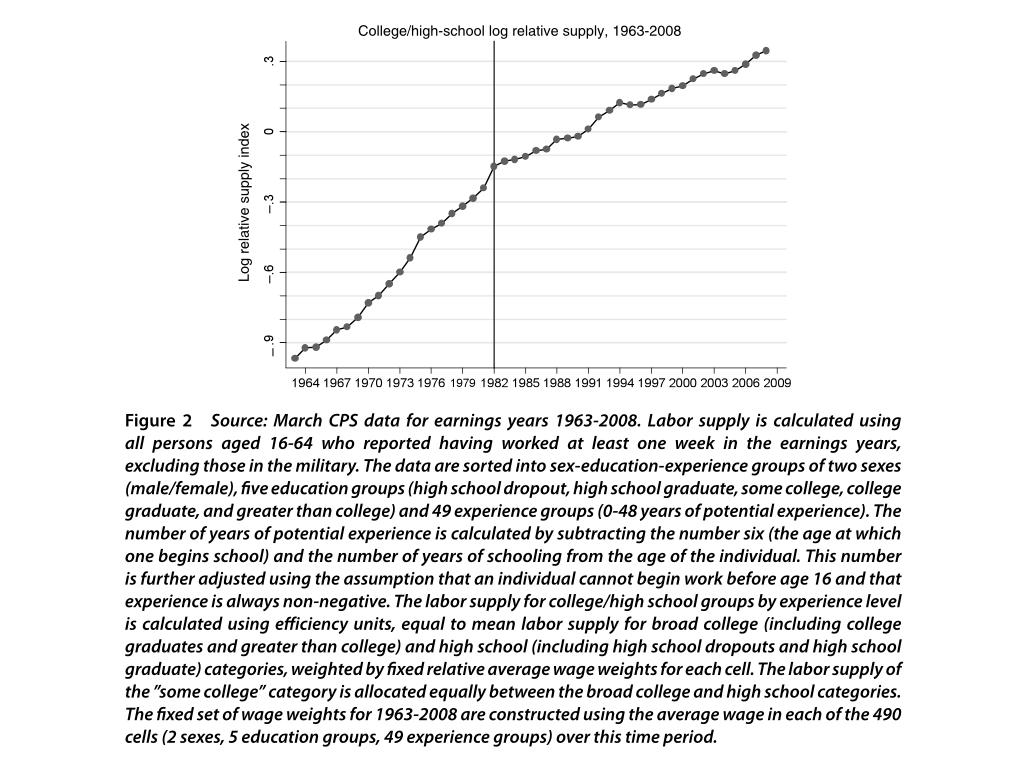
\includegraphics[height=8.5cm,width=\textwidth]{figure2.png}
\end{figure} 
\end{center}
\newpage

\newpage
\begin{center}
\begin{figure}
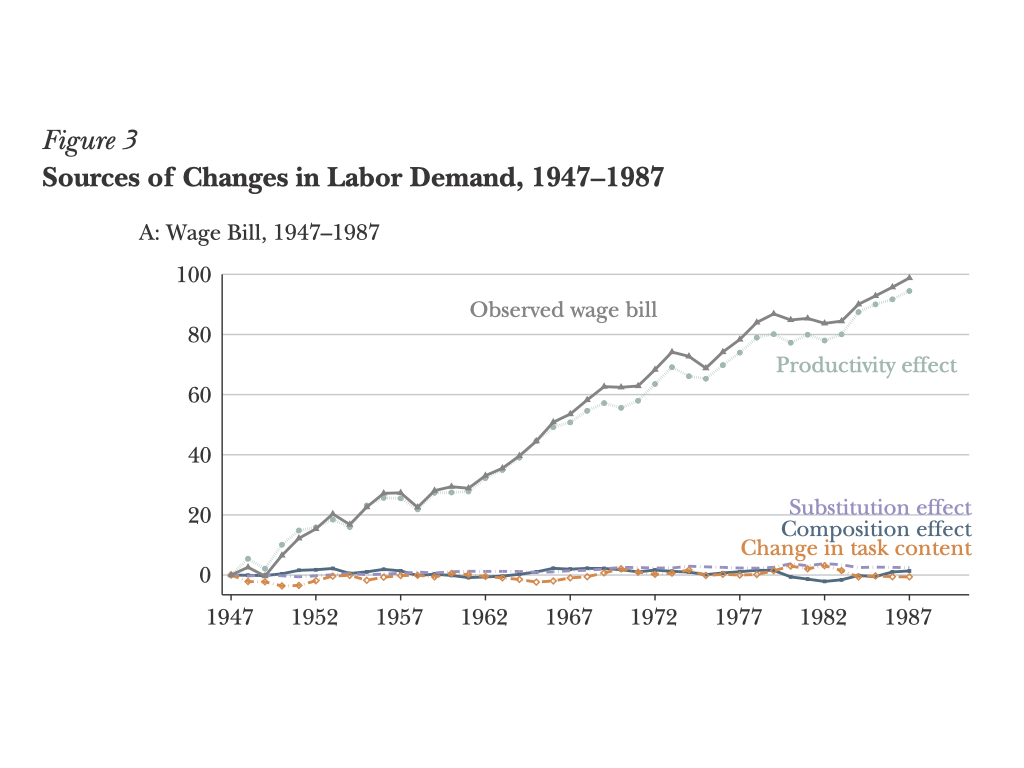
\includegraphics[height=8.5cm,width=\textwidth]{figure3a.png}
\end{figure} 
\end{center}
\newpage

\newpage
\begin{center}
\begin{figure}
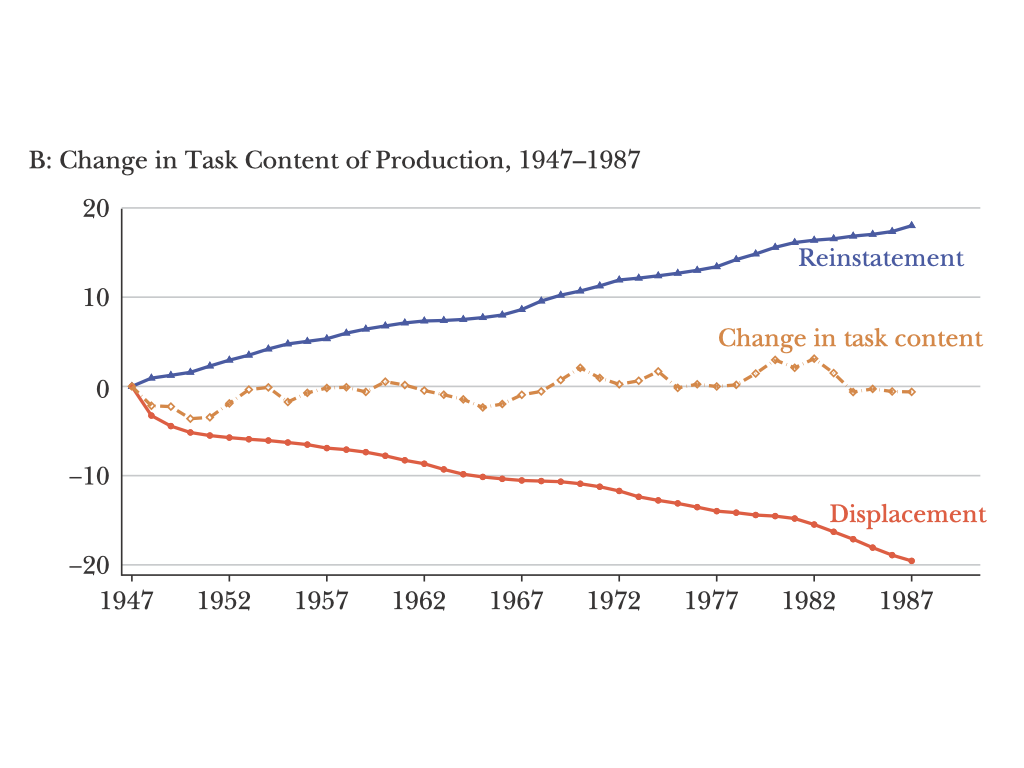
\includegraphics[height=8.5cm,width=\textwidth]{figure3b.png}
\end{figure} 
\end{center}
\newpage

\newpage
\begin{center}
\begin{figure}
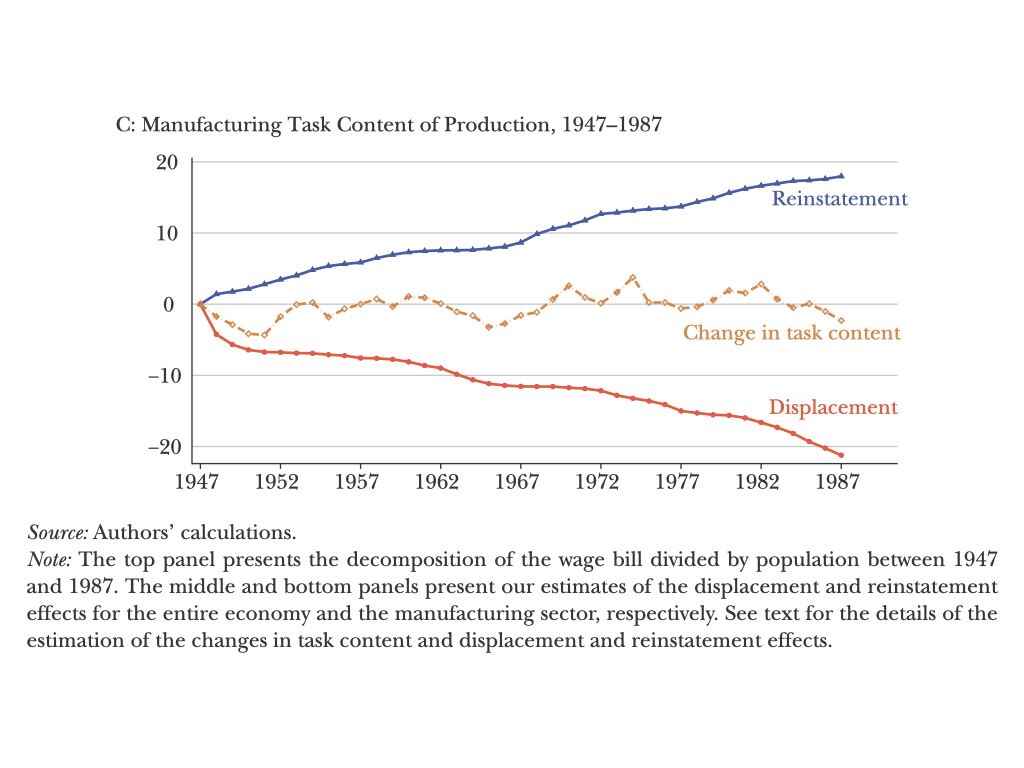
\includegraphics[height=8.5cm,width=\textwidth]{figure3c.png}
\end{figure} 
\end{center}
\newpage

\subsection{2.2 Sources of labor demand: 1987-2017}

\begin{frame}{2. Sources of Labor Demand Growth in the United States}
\begin{itemize}
\item[\textcolor{gray}{2.1}] \textcolor{gray}{Sources of labor demand: 1947-1987} \medskip
\item[\textcolor{red}{2.2}] \textcolor{red}{Sources of labor demand: 1987-2017} \medskip
\item[\textcolor{gray}{2.3}] \textcolor{gray}{What does the change in task content capture?} \medskip
\item[\textcolor{gray}{2.4}] \textcolor{gray}{Confounding factors} \medskip
\item[\textcolor{gray}{2.5}] \textcolor{gray}{What explains the changing nature of technology and slow productivity growth since 1987?} 
\end{itemize}
\end{frame}

\newpage
\begin{center}
\begin{figure}
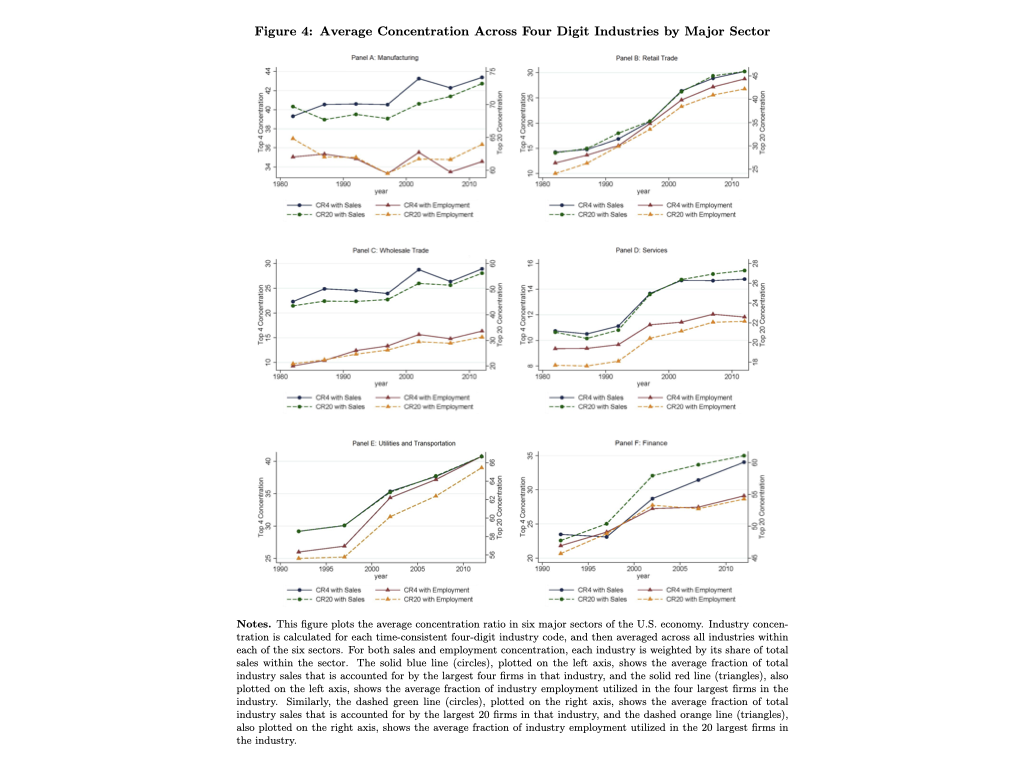
\includegraphics[height=8.5cm,width=\textwidth]{figure4.png}
\end{figure} 
\end{center}
\newpage

\newpage
\begin{center}
\begin{figure}
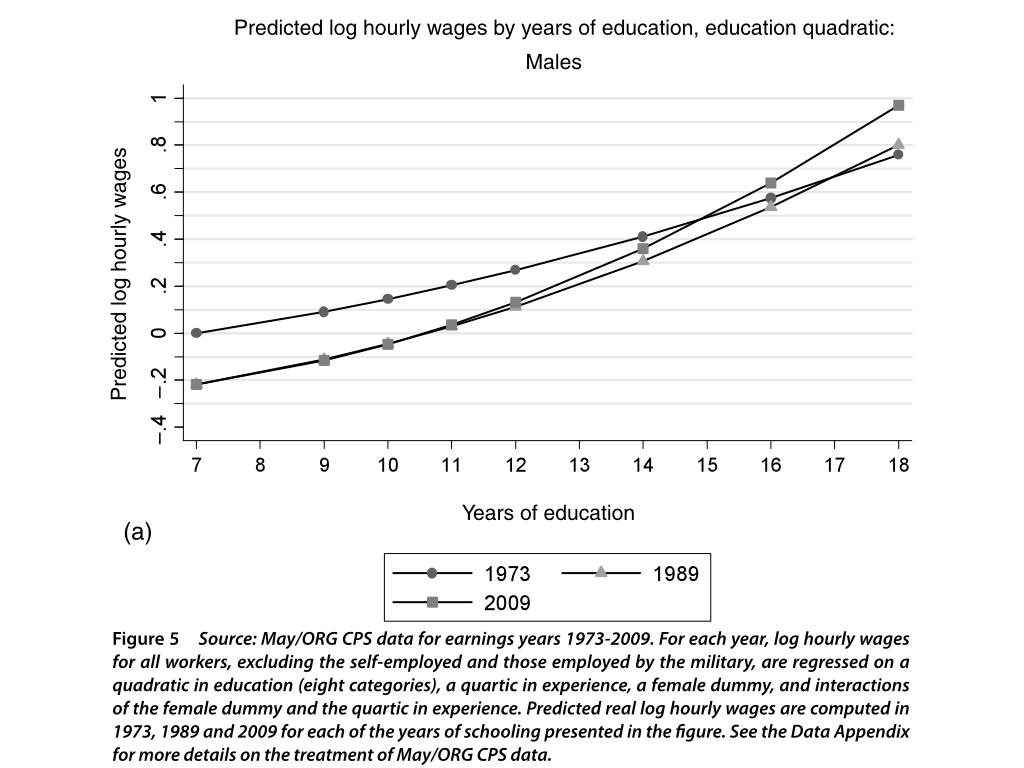
\includegraphics[height=8.5cm,width=\textwidth]{figure5a.png}
\end{figure} 
\end{center}
\newpage

\newpage
\begin{center}
\begin{figure}
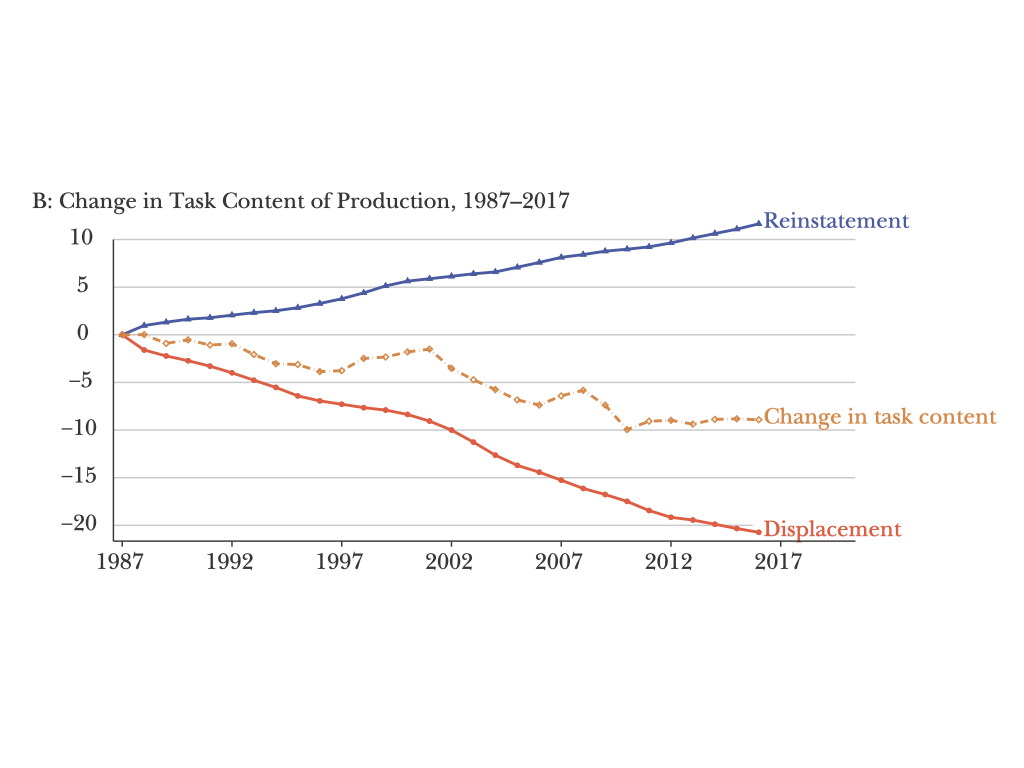
\includegraphics[height=8.5cm,width=\textwidth]{figure5b.png}
\end{figure} 
\end{center}
\newpage

\newpage
\begin{center}
\begin{figure}
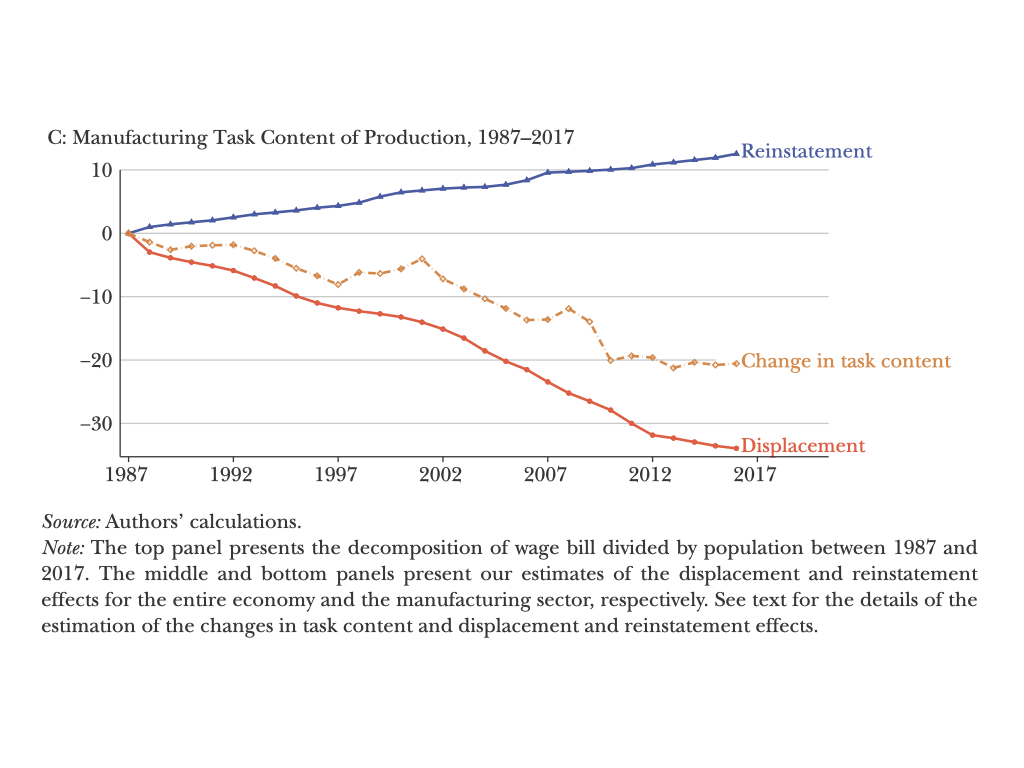
\includegraphics[height=8.5cm,width=\textwidth]{figure5c.png}
\end{figure} 
\end{center}
\newpage

\subsection{2.3 What does the change in task content capture?}

\begin{frame}{2. Sources of Labor Demand Growth in the United States}
\begin{itemize}
\item[\textcolor{gray}{2.1}] \textcolor{gray}{Sources of labor demand: 1947-1987} \medskip
\item[\textcolor{gray}{2.2}] \textcolor{gray}{Sources of labor demand: 1987-2017} \medskip
\item[\textcolor{red}{2.3}] \textcolor{red}{What does the change in task content capture?} \medskip
\item[\textcolor{gray}{2.4}] \textcolor{gray}{Confounding factors} \medskip
\item[\textcolor{gray}{2.5}] \textcolor{gray}{What explains the changing nature of technology and slow productivity growth since 1987?} 
\end{itemize}
\end{frame}

\begin{frame}{Changing task content and automation}
\begin{itemize}
\item The measured change in task content might capture something different than the impact of $dI$. \medskip
\item Correlate changes in task content with other proxies for industry automation for 1987-2014 (Figure A4): \medskip
\begin{enumerate}
\item The penetration of robots in 19 (manufacturing) industries. \medskip
\item The share of routine jobs in 1990. \medskip
\item The share of firms across 148 manufacturing industries using automation technologies.
\end{enumerate}
\end{itemize}
\end{frame}

\newpage
\begin{center}
\begin{figure}
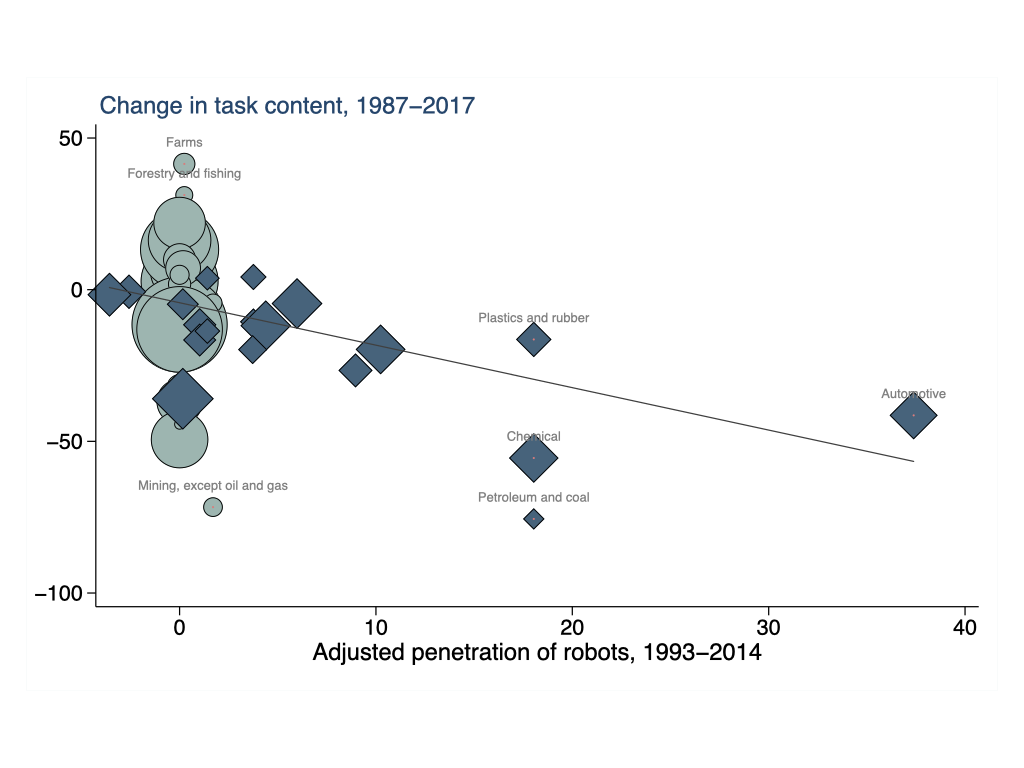
\includegraphics[height=8.5cm,width=\textwidth]{figureA4-1.png}
\end{figure} 
\end{center}
\newpage

\newpage
\begin{center}
\begin{figure}
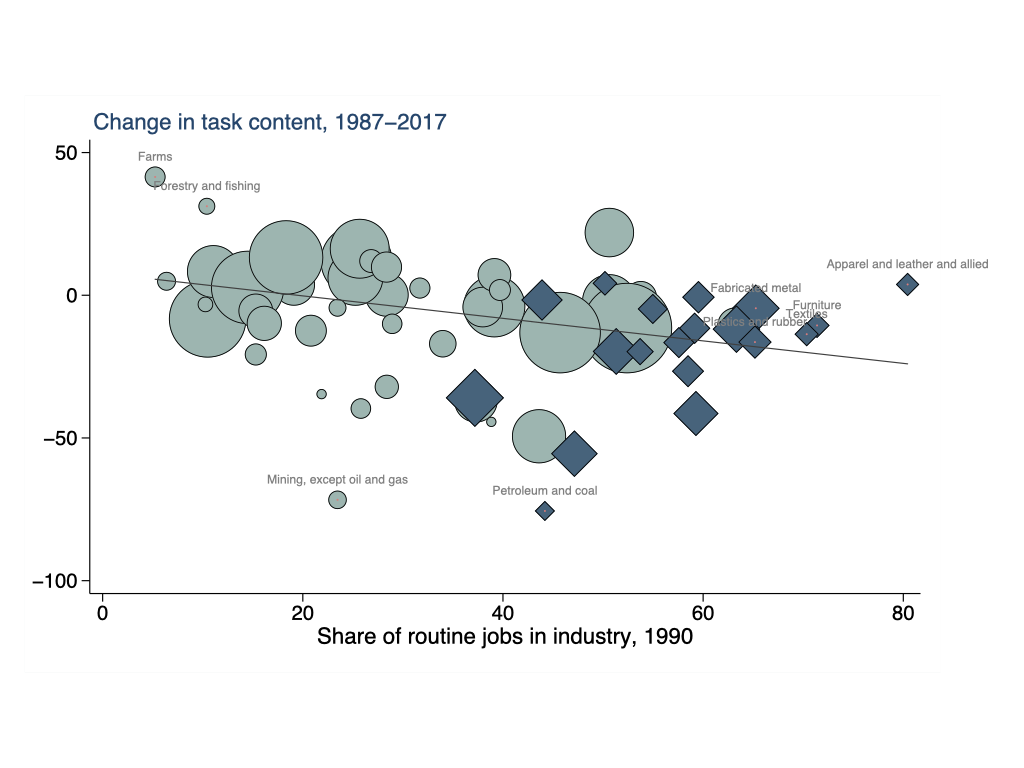
\includegraphics[height=8.5cm,width=\textwidth]{figureA4-2.png}
\end{figure} 
\end{center}
\newpage

\newpage
\begin{center}
\begin{figure}
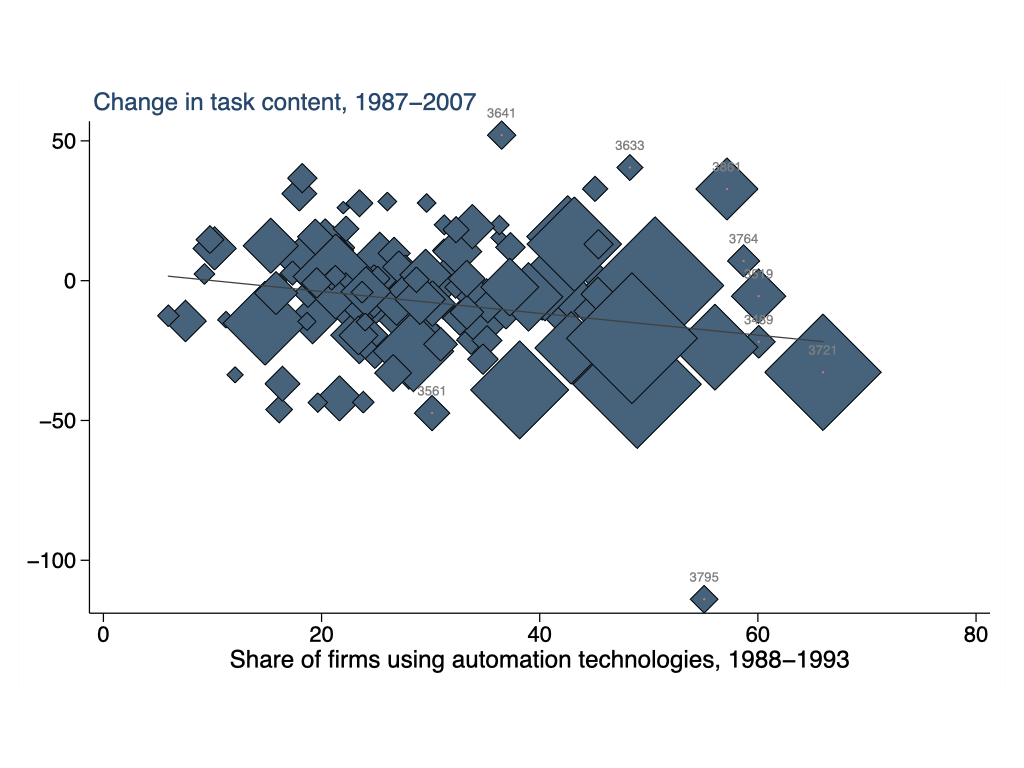
\includegraphics[height=8.5cm,width=\textwidth]{figureA4-3.png}
\end{figure} 
\end{center}
\newpage

\newpage
\begin{center}
\begin{figure}
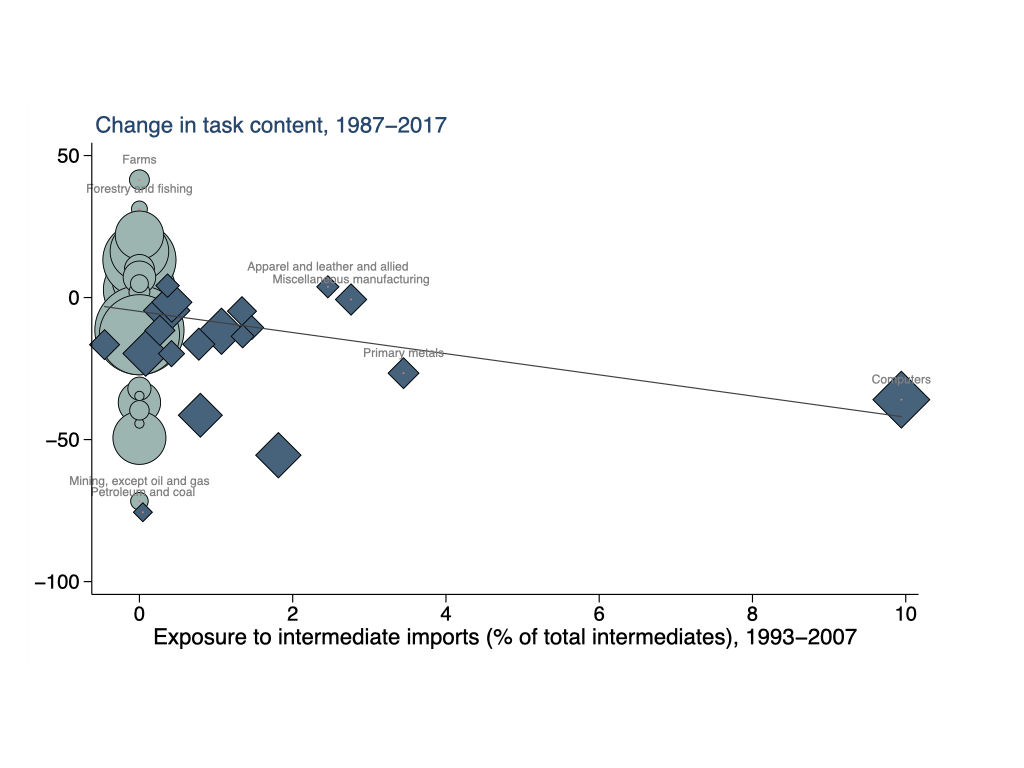
\includegraphics[height=8.5cm,width=\textwidth]{figureA4-4.png}
\end{figure} 
\end{center}
\newpage

\newpage
\begin{center}
\begin{figure}
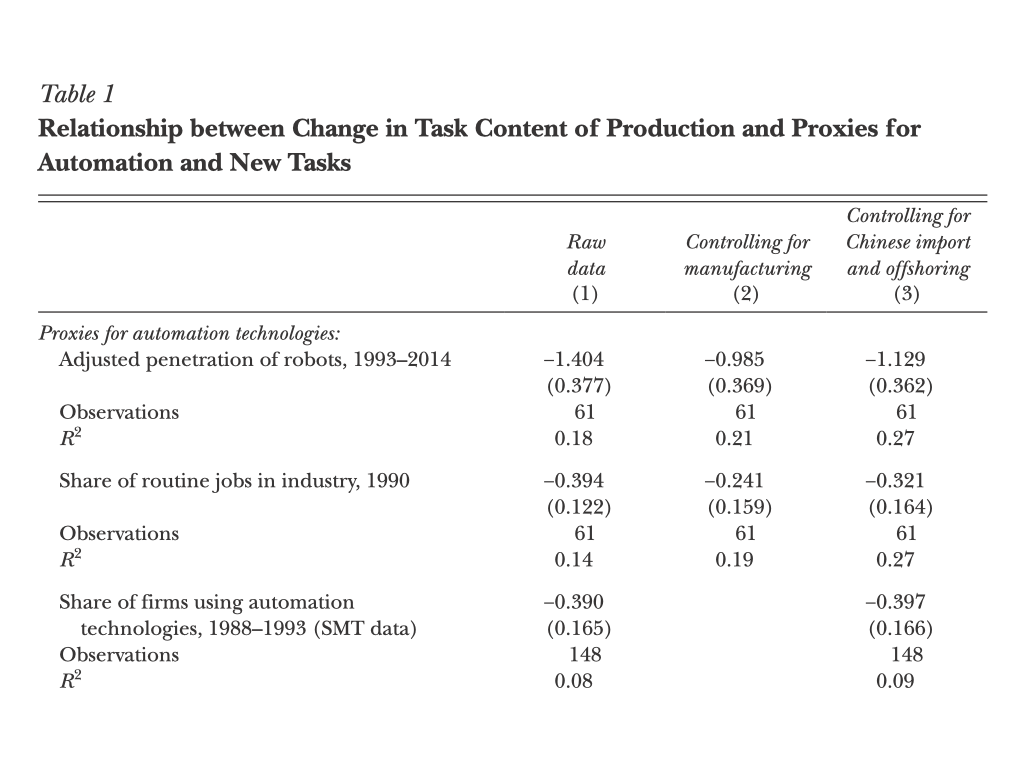
\includegraphics[height=8.5cm,width=\textwidth]{table1-1.png}
\end{figure} 
\end{center}
\newpage

\begin{frame}{Changing task content and creation of new tasks}
Similarly, correlate changes in task content with proxies for new task creation for 1987-2014 (Figure A5): \smallskip
\begin{enumerate}
\item The 1990 share of employment in occupations with a large fraction of new job titles using 1991 DOT. \smallskip
\item The 1990 share of employment in occupations with a large number of ``emerging tasks'' according to O*NET. \smallskip
\item The share of employment growth in an industry accounted for by ``new occupations'' present in 2016 but not in 1990. \smallskip
\item The percent increase in the number of occupations in an industry between 1990 and 2016.
\end{enumerate}
\end{frame}

\newpage
\begin{center}
\begin{figure}
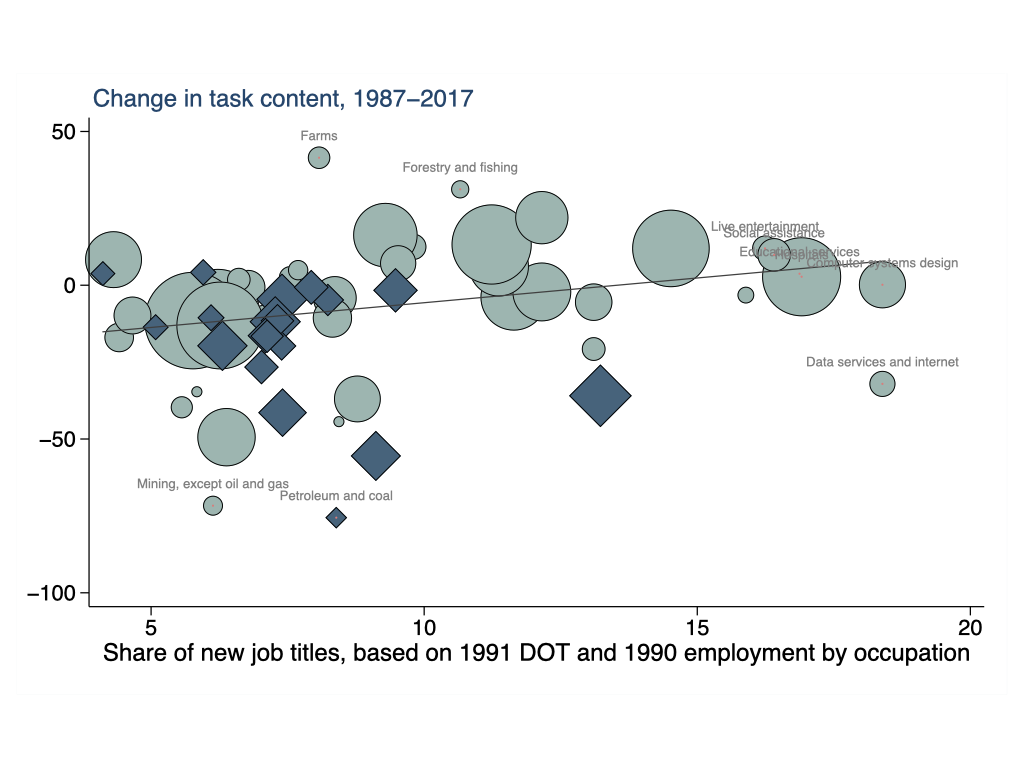
\includegraphics[height=8.5cm,width=\textwidth]{figureA5-1.png}
\end{figure} 
\end{center}
\newpage

\newpage
\begin{center}
\begin{figure}
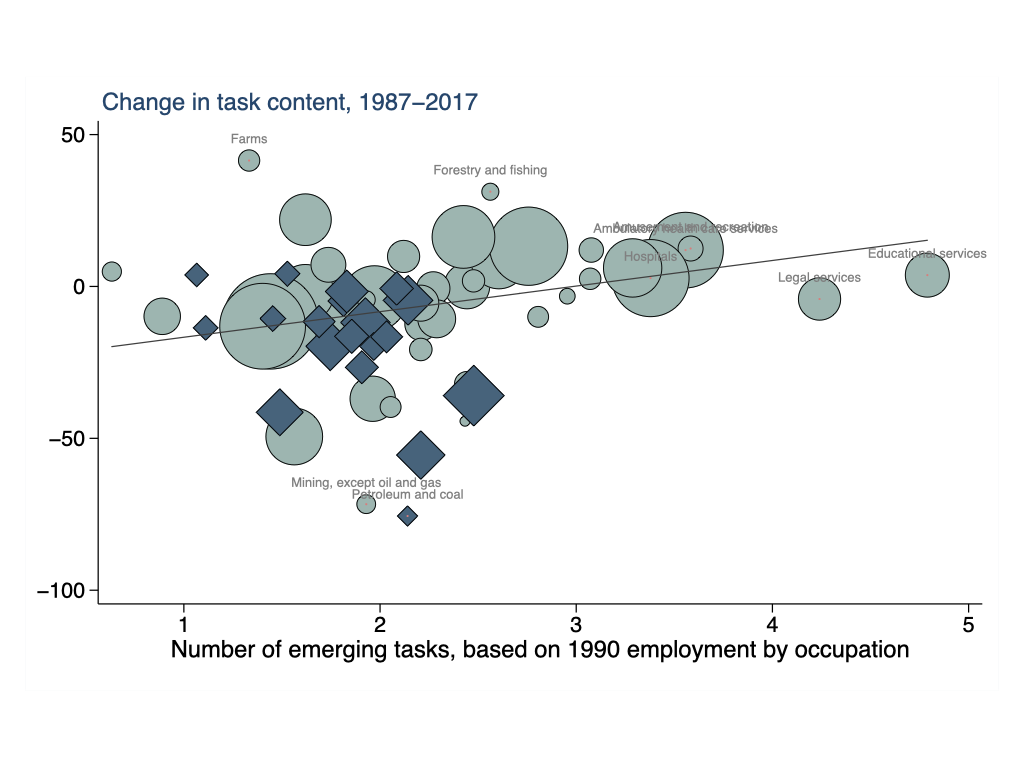
\includegraphics[height=8.5cm,width=\textwidth]{figureA5-2.png}
\end{figure} 
\end{center}
\newpage

\newpage
\begin{center}
\begin{figure}
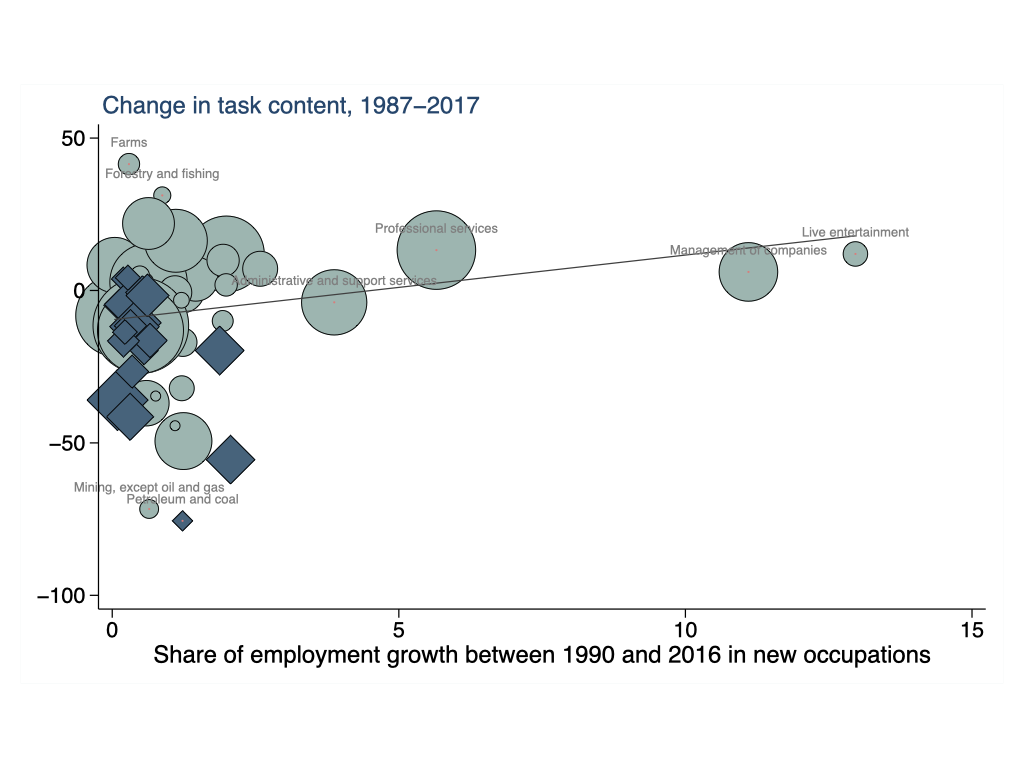
\includegraphics[height=8.5cm,width=\textwidth]{figureA5-3.png}
\end{figure} 
\end{center}
\newpage

\newpage
\begin{center}
\begin{figure}
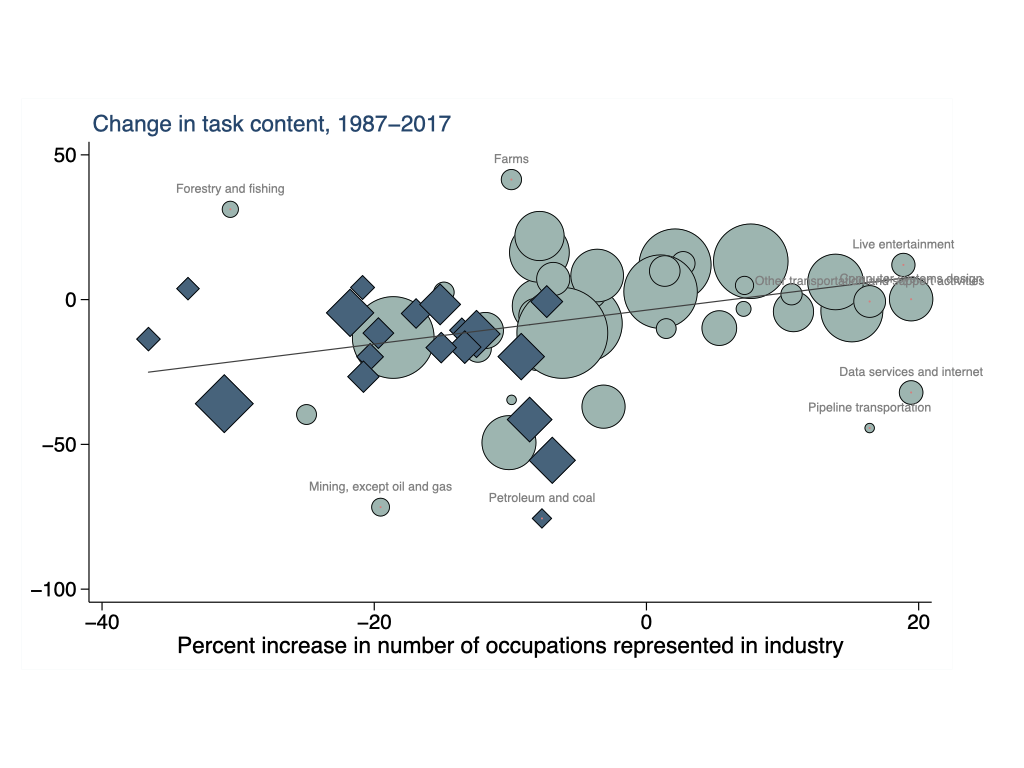
\includegraphics[height=8.5cm,width=\textwidth]{figureA5-4.png}
\end{figure} 
\end{center}
\newpage

\newpage
\begin{center}
\begin{figure}
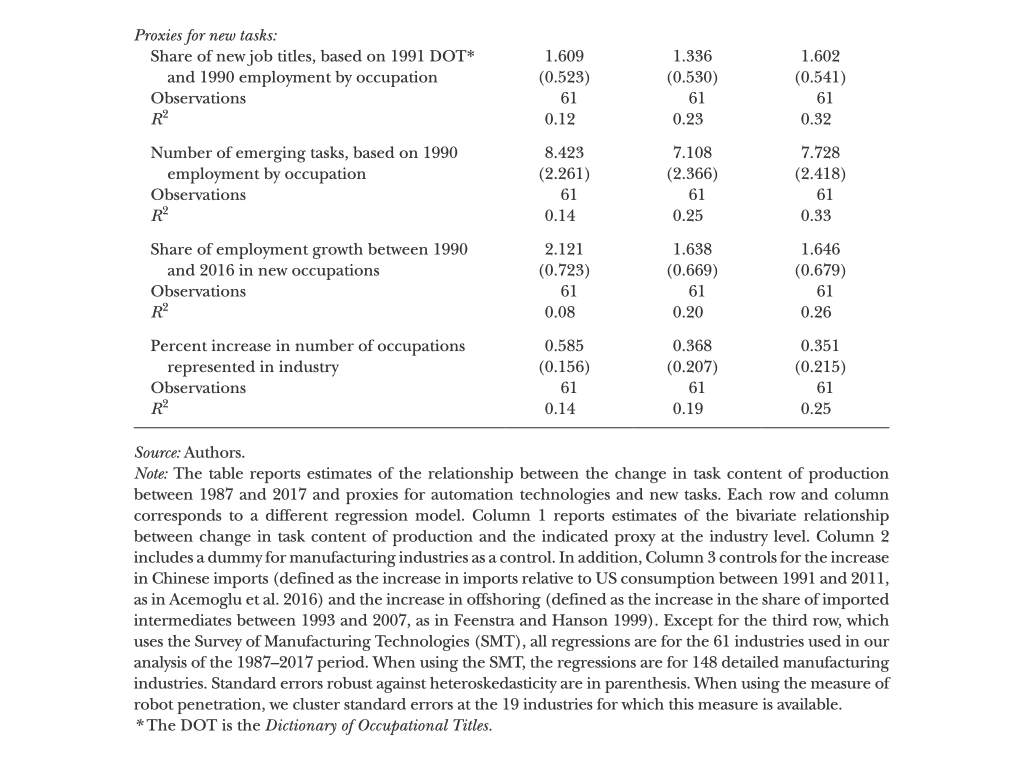
\includegraphics[height=8.5cm,width=\textwidth]{table1-2.png}
\end{figure} 
\end{center}
\newpage

\subsection{2.4 Confounding factors}

\begin{frame}{2. Sources of Labor Demand Growth in the United States}
\begin{itemize}
\item[\textcolor{gray}{2.1}] \textcolor{gray}{Sources of labor demand: 1947-1987} \medskip
\item[\textcolor{gray}{2.2}] \textcolor{gray}{Sources of labor demand: 1987-2017} \medskip
\item[\textcolor{gray}{2.3}] \textcolor{gray}{What does the change in task content capture?} \medskip
\item[\textcolor{red}{2.4}] \textcolor{red}{Confounding factors} \medskip
\item[\textcolor{gray}{2.5}] \textcolor{gray}{What explains the changing nature of technology and slow productivity growth since 1987?} 
\end{itemize}
\end{frame}

\begin{frame}{Confounding factors}
\begin{itemize}
\item \underline{Trade in final goods} is captured by the productivity and composition effects (see Table 1). \medskip
\item \underline{Offshoring} changing task content does not seem important (see Table 1). \medskip
\item \underline{Structural change} is captured by the composition effect.  \medskip
\item \underline{Demographic changes} (e.g. skill-upgrading, participation, aging) are captured by the substitution effect. \medskip
\item \underline{Imperfections} (e.g. bargaining, rent-sharing) are allowed as long as we remain on the labor demand curve.
\end{itemize}
\end{frame}

\subsection{2.5 What explains the changing nature of technology and slow productivity growth since 1987?}

\begin{frame}{2. Sources of Labor Demand Growth in the United States}
\begin{itemize}
\item[\textcolor{gray}{2.1}] \textcolor{gray}{Sources of labor demand: 1947-1987} \medskip
\item[\textcolor{gray}{2.2}] \textcolor{gray}{Sources of labor demand: 1987-2017} \medskip
\item[\textcolor{gray}{2.3}] \textcolor{gray}{What does the change in task content capture?} \medskip
\item[\textcolor{gray}{2.4}] \textcolor{gray}{Confounding factors} \medskip
\item[\textcolor{red}{2.5}] \textcolor{red}{What explains the changing nature of technology and slow productivity growth since 1987?} 
\end{itemize}
\end{frame}

\begin{frame}{Why has the nature of technological progress changed?}
\begin{itemize}
\item The innovation possibilities frontier may have shifted, facilitating automation and making the creation of new labor-intensive tasks more difficult (e.g. AI). \medskip
\item Tax incentives for automation have increased relative to the creation of new labor-intensive tasks. \medskip
\item Increasing market power of large tech companies with business models based on automation and small workforces. \medskip
\item Declining government support for innovation with longer horizons (given that technologies that create new tasks bear fruit more slowly).
\end{itemize}
\end{frame}

\section{3. Concluding Remarks}

\begin{frame}{3. Concluding Remarks}
\begin{itemize}
\item This paper develops the most complete (and accessible) task-based model to study the effects of different technologies on labor demand. \medskip
\item Automation shifts task content against labor, while the creation of new tasks improves it. \medskip
\item These technologies are qualitatively different from factor-augmenting ones. \medskip
\item Changes in task content can be inferred from data on labor shares, value added, and factor prices at the industry level.
\end{itemize}
\end{frame}

\end{document}
